% !TeX document-id = {50f0f04c-d5f8-4417-bb49-0e71ddd7bfde}
% !TeX TXS-program:bibliography = txs:///biber

\documentclass[conference]{IEEEtran}
%\IEEEoverridecommandlockouts
% The preceding line is only needed to identify funding in the first footnote. If that is unneeded, please comment it out.
%\usepackage{cite}
\usepackage{amsmath,amssymb,amsfonts}
\usepackage{algorithmic}
\usepackage{graphicx}
\usepackage{textcomp}
\usepackage{xcolor}
\usepackage{tikz}
\usetikzlibrary{arrows.meta}
\usetikzlibrary{chains}
\usetikzlibrary {matrix}
\usepackage{fontawesome5}
\usepackage{enumitem}
\usepackage{hyperref}
\usepackage[%
  bibstyle=ieee,
  citestyle=numeric,
  isbn=true,
  doi=false,
  sorting=none,
  url=true,
  defernumbers=true,
  bibencoding=utf8,
  backend=biber
]{biblatex}
\addbibresource{bibliography.bib}
%\usepackage{siunitx}

%% TODONOTES
\paperwidth=\dimexpr \paperwidth + 6cm\relax
\oddsidemargin=\dimexpr\oddsidemargin + 3cm\relax
\evensidemargin=\dimexpr\evensidemargin + 3cm\relax
\marginparwidth=\dimexpr \marginparwidth + 3cm\relax
\usepackage{todonotes}


% Key-system

\newcommand{\ptpperfLoadKeys}[1]{\pgfkeys{#1}}
\newcommand{\ptpKeyPrefix}{/ptpperf}
\newcommand{\ptpKey}[1]{\pgfkeysifdefined{\ptpKeyPrefix/#1}{\pgfkeysvalueof{\ptpKeyPrefix/#1}}{0}}
\newcommand{\fTime}[2][0]{\fpeval{round((#2) * 10e5, #1)}\,\textmu{}s}
\newcommand{\fTimeMS}[2][0]{\fpeval{round((#2) * 10e2, #1)}\,ms}
\newcommand{\fTimeMin}[2][0]{\fpeval{round((#2) / 60, #1)}\,min}
\newcommand{\fTimeKey}[2][0]{\fTime[#1]{\ptpKey{#2}}}
\newcommand{\fTimeMath}[2][0]{\fTime{\fpeval{round(#2, #1)}}}
\newcommand{\fNum}[2][0]{\fpeval{round(#2, #1)}}
\newcommand{\fRatio}[2][0]{\fpeval{round(#2, #1)}$\times$}
\newcommand{\fPercentage}[2][0]{\fpeval{round(100*(#2), #1)}\%}
\newcommand{\fRelative}[2][0]{\fpeval{round(100*(#2)-100, #1)}\%}
\newcommand{\fRelativeInverted}[2][0]{\fpeval{100-round(100*(#2), #1)}\%}

% Format vendor ids to names
\pgfkeys{
    /ptpperf/vendors/.cd,
    ptpd/.initial={PTPd},
    linuxptp/.initial={LinuxPTP},
    sptp/.initial={SPTP},
    chrony/.initial={Chrony},
    /ptpperf/clusters/.cd,
    rpi-4/.initial={Raspberry-Pi 4},
    rpi-5/.initial={Raspberry-Pi 5},
    /ptpperf/vendorcluster/.cd,
    ptpd/rpi-4/.initial={PTPd on Raspberry-Pi 4},
    linuxptp/rpi-4/.initial={LinuxPTP on Raspberry-Pi 4},
    sptp/rpi-4/.initial={SPTP on Raspberry-Pi 4},
    chrony/rpi-4/.initial={Chrony on Raspberry-Pi 4},
    ptpd/rpi-5/.initial={PTPd on Raspberry-Pi 5},
    linuxptp/rpi-5/.initial={LinuxPTP on Raspberry-Pi 5},
    sptp/rpi-5/.initial={SPTP on Raspberry-Pi 5},
    chrony/rpi-5/.initial={Chrony on Raspberry-Pi 5},
}
\newcommand{\fVendor}[1]{\pgfkeysvalueof{/ptpperf/vendors/#1}}
\newcommand{\fCluster}[1]{\pgfkeysvalueof{/ptpperf/clusters/#1}}
\newcommand{\fVendorCluster}[1]{\pgfkeysvalueof{/ptpperf/vendorcluster/#1}}
\newcommand{\vendors}{ptpd,linuxptp,sptp,chrony}

% Comparison Tools

\newcommand{\cmpMin}{}
\newcommand{\cmpMinArg}{}
\newcommand{\cmpMax}{}
\newcommand{\cmpMaxArg}{}
\newcommand{\cmpMean}{}
\newcommand{\cmpCount}{}

% Search for a value: #1: counter macro, #2: values, #3: optimization functio (min/max), #4: Function value to calculate
\newcommand{\cmpSearch}[3]{%
    \xdef\cmpMin{}%
    \xdef\cmpMinArg{}%
    \xdef\cmpMax{}%
    \xdef\cmpMaxArg{}%
    \xdef\cmpMean{}%
    \xdef\cmpCount{0}%
    % Loop across values searching for the best one
    \foreach #1 in {#2}{%
        \xdef\currentValue{\fpeval{#3}}%
        %
        % If first iteration, then define best value.
        \ifundef{\cmpMin}{\xdef\cmpMin{\currentValue}}{}%
        \ifundef{\cmpMax}{\xdef\cmpMax{\currentValue}}{}%
        %
        % Update best value and if changed, then also update best argument.
        \xdef\cmpMin{\fpeval{min(\currentValue, \cmpMin)}}%
        \strcmpfullexpand{\currentValue}{\cmpMin}{\xdef\cmpMinArg{#1}}{}%
        %
        % Same for max.
        \xdef\cmpMax{\fpeval{max(\currentValue, \cmpMax)}}%
        \strcmpfullexpand{\currentValue}{\cmpMax}{\xdef\cmpMaxArg{#1}}{}%
        %
        \xdef\cmpMean{\fpeval{\cmpMean + \currentValue}}%
        \xdef\cmpCount{\fpeval{\cmpCount + 1}}%
%        Trace: \vendor, \currentValue, \cmpValue, \cmpArg\\
    }%
    %
    \xdef\cmpMean{\fpeval{\cmpMean/\cmpCount}}
}

\newcommand{\cmpSearchVendor}[1]{\cmpSearch{\vendor}{ptpd,linuxptp,sptp,chrony}{#1}}
\newcommand{\cmpSearchVendorCluster}[1]{\cmpSearch{\vendor/\cluster}{ptpd/rpi-4,linuxptp/rpi-4,sptp/rpi-4,chrony/rpi-4,ptpd/rpi-5,linuxptp/rpi-5,sptp/rpi-5,chrony/rpi-5}{#1}}
\newcommand{\cmpSave}[1]{%
    \pgfkeys{
        \ptpKeyPrefix/cmp/.cd,
        #1/min/.initial/.expanded={\cmpMin},
        #1/minarg/.initial/.expanded={\cmpMinArg},
        #1/max/.initial/.expanded={\cmpMax},
        #1/maxarg/.initial/.expanded={\cmpMaxArg},
        #1/mean/.initial/.expanded={\cmpMean},
    }%
}
\newcommand{\cmpLoad}[1]{%
    \xdef\cmpMin{\ptpKey{cmp/#1/min}}%
    \xdef\cmpMinArg{\ptpKey{cmp/#1/minarg}}%
    \xdef\cmpMax{\ptpKey{cmp/#1/max}}%
    \xdef\cmpMaxArg{\ptpKey{cmp/#1/maxarg}}%
    \xdef\cmpMean{\ptpKey{cmp/#1/mean}}%
}
\newcommand{\cmpKey}[2]{\ptpKey{cmp/#1/#2}}
\newcommand{\cmpRatioVendorClusterVsBaseline}[1]{\ptpKey{#1/\cluster/\vendor/q50}/\ptpKey{base/\cluster/\vendor/q50}}

\newcommand{\assertError}[1]{\textbf{\textcolor{red}{ASSERTION ERROR: #1}}\errmessage{ASSERTION ERROR: #1}}
% Raise an error if #2 != #3, with optional message #1.
\newcommand{\assert}[3][]{\strcmpfullexpand{#2}{#3}{}{\assertError{\strcmpfullexpand{#1}{}{#2 != #3}{#1}}}}
\newcommand{\assertRange}[3]{\pgfmathparse{ifthenelse(and(\fpeval{#1} >= #2, \fpeval{#1} <= #3),"1","0")}\assert[\fpeval{#1} not in range (#2, #3)]{\pgfmathresult}{1}}

% Utility

\makeatletter
\newcommand*{\strcmpfullexpand}[4]{%
  \ifnum\pdf@strcmp{#1}{#2}=\z@#3\else#4\fi%
}
\makeatother

\begin{document}

\title{Telling the Time: Modern-Day Complications}
%\thanks{Identify applicable funding agency here. If none, delete this.}

\author{\IEEEauthorblockN{Vincent Bode}
\IEEEauthorblockA{\textit{Department of Computer Science} \\
\textit{Technical University of Munich}\\
Munich, Germany \\
vincent.bode@tum.de}
\and
\IEEEauthorblockN{Arpan Gujarati}
\IEEEauthorblockA{\textit{Department of Computer Science} \\
\textit{University of British Columbia}\\
Vancouver, Canada \\
arpanbg@cs.ubc.ca}
%\and
%\IEEEauthorblockN{3\textsuperscript{rd} Given Name Surname}
%\IEEEauthorblockA{\textit{dept. name of organization (of Aff.)} \\
%\textit{name of organization (of Aff.)}\\
%City, Country \\
%email address or ORCID}
}

\maketitle

\textbf{Potential Targets:}

\begin{tabular}{p{5cm}l}
    Venue & Deadline\\
    \href{https://ieee-ims.org/document/ispcs-2024-call-papers}{Symposium on Precision Clock Synchronization for Measurement, Control, \& Communication} & 20.03.2024\\
    \href{https://2024.rtss.org/call-for-papers/}{RTSS} & 23.05.2024\\
    \href{https://2024.rtss.org/call-for-papers/}{SIGMETRICS} & 02.08.2023 (first of 3)\\
    \href{https://ieee-ims.org/document/i2mtc-2024-call-papers}{Instrumentation and Measurement Technology Conference} & 24.11.2023\\
\end{tabular}

\begin{abstract}
\end{abstract}

\begin{IEEEkeywords}
PTP, Time Synchronization, Fault Tolerance
\end{IEEEkeywords}

\ptpperfLoadKeys{
    /ptpperf/base/rpi-4/chrony/pd/q5/.initial=0.0001117,
    /ptpperf/base/rpi-4/chrony/pd/q50/.initial=0.0001217,
    /ptpperf/base/rpi-4/chrony/pd/q95/.initial=0.000132,
    /ptpperf/base/rpi-4/chrony/q5/.initial=1.1900000000000001e-07,
    /ptpperf/base/rpi-4/chrony/q50/.initial=1.325e-06,
    /ptpperf/base/rpi-4/chrony/q95/.initial=4.808600000000004e-06,
    /ptpperf/base/rpi-4/linuxptp/pd/q5/.initial=6.1473e-05,
    /ptpperf/base/rpi-4/linuxptp/pd/q50/.initial=6.449900000000001e-05,
    /ptpperf/base/rpi-4/linuxptp/pd/q95/.initial=6.948525e-05,
    /ptpperf/base/rpi-4/linuxptp/q5/.initial=5.2725e-07,
    /ptpperf/base/rpi-4/linuxptp/q50/.initial=5.0169999999999996e-06,
    /ptpperf/base/rpi-4/linuxptp/q95/.initial=1.50795e-05,
    /ptpperf/base/rpi-4/ptpd/pd/q5/.initial=7.1771e-05,
    /ptpperf/base/rpi-4/ptpd/pd/q50/.initial=7.922200000000001e-05,
    /ptpperf/base/rpi-4/ptpd/pd/q95/.initial=9.206459999999999e-05,
    /ptpperf/base/rpi-4/ptpd/q5/.initial=6.016000000000001e-07,
    /ptpperf/base/rpi-4/ptpd/q50/.initial=7.395e-06,
    /ptpperf/base/rpi-4/ptpd/q95/.initial=4.5662000000000004e-05,
    /ptpperf/base/rpi-4/sptp/pd/q5/.initial=6.288935e-05,
    /ptpperf/base/rpi-4/sptp/pd/q50/.initial=6.8223e-05,
    /ptpperf/base/rpi-4/sptp/pd/q95/.initial=7.629615e-05,
    /ptpperf/base/rpi-4/sptp/q5/.initial=2.08e-07,
    /ptpperf/base/rpi-4/sptp/q50/.initial=2.4485000000000004e-06,
    /ptpperf/base/rpi-4/sptp/q95/.initial=7.866249999999998e-06,
    /ptpperf/base/rpi-5/chrony/pd/q5/.initial=7.439000000000001e-05,
    /ptpperf/base/rpi-5/chrony/pd/q50/.initial=7.509e-05,
    /ptpperf/base/rpi-5/chrony/pd/q95/.initial=7.578000000000001e-05,
    /ptpperf/base/rpi-5/chrony/q5/.initial=1.4000000000000001e-08,
    /ptpperf/base/rpi-5/chrony/q50/.initial=1.7600000000000001e-07,
    /ptpperf/base/rpi-5/chrony/q95/.initial=5.09e-07,
    /ptpperf/base/rpi-5/linuxptp/pd/q5/.initial=3.6584e-05,
    /ptpperf/base/rpi-5/linuxptp/pd/q50/.initial=3.6779e-05,
    /ptpperf/base/rpi-5/linuxptp/pd/q95/.initial=3.6963850000000004e-05,
    /ptpperf/base/rpi-5/linuxptp/q5/.initial=2.8000000000000003e-08,
    /ptpperf/base/rpi-5/linuxptp/q50/.initial=3.2600000000000003e-07,
    /ptpperf/base/rpi-5/linuxptp/q95/.initial=8.790000000000001e-07,
    /ptpperf/base/rpi-5/ptpd/pd/q5/.initial=0.00011537500000000001,
    /ptpperf/base/rpi-5/ptpd/pd/q50/.initial=0.000116031,
    /ptpperf/base/rpi-5/ptpd/pd/q95/.initial=0.000116625,
    /ptpperf/base/rpi-5/ptpd/q5/.initial=1.01e-07,
    /ptpperf/base/rpi-5/ptpd/q50/.initial=1.13e-06,
    /ptpperf/base/rpi-5/ptpd/q95/.initial=3.668349999999999e-06,
    /ptpperf/base/rpi-5/sptp/pd/q5/.initial=7.7229e-05,
    /ptpperf/base/rpi-5/sptp/pd/q50/.initial=7.8309e-05,
    /ptpperf/base/rpi-5/sptp/pd/q95/.initial=7.9466e-05,
    /ptpperf/base/rpi-5/sptp/q5/.initial=4.6e-08,
    /ptpperf/base/rpi-5/sptp/q50/.initial=5.03e-07,
    /ptpperf/base/rpi-5/sptp/q95/.initial=1.6650000000000002e-06,
    /ptpperf/load/cpu_prioritized/load_100/rpi-4/chrony/pd/q5/.initial=0.0001173,
    /ptpperf/load/cpu_prioritized/load_100/rpi-4/chrony/pd/q50/.initial=0.0001229,
    /ptpperf/load/cpu_prioritized/load_100/rpi-4/chrony/pd/q95/.initial=0.0001365,
    /ptpperf/load/cpu_prioritized/load_100/rpi-4/chrony/q5/.initial=1.1500000000000001e-07,
    /ptpperf/load/cpu_prioritized/load_100/rpi-4/chrony/q50/.initial=1.3240000000000002e-06,
    /ptpperf/load/cpu_prioritized/load_100/rpi-4/chrony/q95/.initial=6.024e-06,
    /ptpperf/load/cpu_prioritized/load_100/rpi-4/linuxptp/pd/q5/.initial=5.9482000000000004e-05,
    /ptpperf/load/cpu_prioritized/load_100/rpi-4/linuxptp/pd/q50/.initial=6.438800000000001e-05,
    /ptpperf/load/cpu_prioritized/load_100/rpi-4/linuxptp/pd/q95/.initial=6.742900000000001e-05,
    /ptpperf/load/cpu_prioritized/load_100/rpi-4/linuxptp/q5/.initial=7.734000000000002e-07,
    /ptpperf/load/cpu_prioritized/load_100/rpi-4/linuxptp/q50/.initial=6.691000000000001e-06,
    /ptpperf/load/cpu_prioritized/load_100/rpi-4/linuxptp/q95/.initial=1.6685599999999998e-05,
    /ptpperf/load/cpu_prioritized/load_100/rpi-4/ptpd/pd/q5/.initial=6.253830000000001e-05,
    /ptpperf/load/cpu_prioritized/load_100/rpi-4/ptpd/pd/q50/.initial=7.2036e-05,
    /ptpperf/load/cpu_prioritized/load_100/rpi-4/ptpd/pd/q95/.initial=7.3966e-05,
    /ptpperf/load/cpu_prioritized/load_100/rpi-4/ptpd/q5/.initial=6.03e-07,
    /ptpperf/load/cpu_prioritized/load_100/rpi-4/ptpd/q50/.initial=6.183000000000001e-06,
    /ptpperf/load/cpu_prioritized/load_100/rpi-4/ptpd/q95/.initial=1.989189999999999e-05,
    /ptpperf/load/cpu_prioritized/load_100/rpi-4/sptp/pd/q5/.initial=6.1464e-05,
    /ptpperf/load/cpu_prioritized/load_100/rpi-4/sptp/pd/q50/.initial=6.480800000000001e-05,
    /ptpperf/load/cpu_prioritized/load_100/rpi-4/sptp/pd/q95/.initial=7.375155e-05,
    /ptpperf/load/cpu_prioritized/load_100/rpi-4/sptp/q5/.initial=1.9300000000000002e-07,
    /ptpperf/load/cpu_prioritized/load_100/rpi-4/sptp/q50/.initial=2.0100000000000002e-06,
    /ptpperf/load/cpu_prioritized/load_100/rpi-4/sptp/q95/.initial=7.308750000000002e-06,
    /ptpperf/load/cpu_prioritized/load_100/rpi-5/chrony/pd/q5/.initial=7.439000000000001e-05,
    /ptpperf/load/cpu_prioritized/load_100/rpi-5/chrony/pd/q50/.initial=7.509e-05,
    /ptpperf/load/cpu_prioritized/load_100/rpi-5/chrony/pd/q95/.initial=7.5766e-05,
    /ptpperf/load/cpu_prioritized/load_100/rpi-5/chrony/q5/.initial=2.2000000000000002e-08,
    /ptpperf/load/cpu_prioritized/load_100/rpi-5/chrony/q50/.initial=2.26e-07,
    /ptpperf/load/cpu_prioritized/load_100/rpi-5/chrony/q95/.initial=7.541999999999976e-07,
    /ptpperf/load/cpu_prioritized/load_100/rpi-5/sptp/pd/q5/.initial=7.799260000000001e-05,
    /ptpperf/load/cpu_prioritized/load_100/rpi-5/sptp/pd/q50/.initial=8.1024e-05,
    /ptpperf/load/cpu_prioritized/load_100/rpi-5/sptp/pd/q95/.initial=8.403235000000001e-05,
    /ptpperf/load/cpu_prioritized/load_100/rpi-5/sptp/q5/.initial=1.2050000000000003e-07,
    /ptpperf/load/cpu_prioritized/load_100/rpi-5/sptp/q50/.initial=1.3425e-06,
    /ptpperf/load/cpu_prioritized/load_100/rpi-5/sptp/q95/.initial=4.2374499999999996e-06,
    /ptpperf/load/cpu_unprioritized/load_100/rpi-4/chrony/pd/q5/.initial=0.00011820000000000001,
    /ptpperf/load/cpu_unprioritized/load_100/rpi-4/chrony/pd/q50/.initial=0.0001242,
    /ptpperf/load/cpu_unprioritized/load_100/rpi-4/chrony/pd/q95/.initial=0.00013800000000000002,
    /ptpperf/load/cpu_unprioritized/load_100/rpi-4/chrony/q5/.initial=1.46e-07,
    /ptpperf/load/cpu_unprioritized/load_100/rpi-4/chrony/q50/.initial=1.5020000000000002e-06,
    /ptpperf/load/cpu_unprioritized/load_100/rpi-4/chrony/q95/.initial=5.959e-06,
    /ptpperf/load/cpu_unprioritized/load_100/rpi-4/linuxptp/pd/q5/.initial=6.232500000000001e-05,
    /ptpperf/load/cpu_unprioritized/load_100/rpi-4/linuxptp/pd/q50/.initial=6.626800000000001e-05,
    /ptpperf/load/cpu_unprioritized/load_100/rpi-4/linuxptp/pd/q95/.initial=6.891300000000001e-05,
    /ptpperf/load/cpu_unprioritized/load_100/rpi-4/linuxptp/q5/.initial=3.7600000000000003e-07,
    /ptpperf/load/cpu_unprioritized/load_100/rpi-4/linuxptp/q50/.initial=4.311e-06,
    /ptpperf/load/cpu_unprioritized/load_100/rpi-4/linuxptp/q95/.initial=1.635269999999999e-05,
    /ptpperf/load/cpu_unprioritized/load_100/rpi-4/ptpd/pd/q5/.initial=6.2168e-05,
    /ptpperf/load/cpu_unprioritized/load_100/rpi-4/ptpd/pd/q50/.initial=6.6201e-05,
    /ptpperf/load/cpu_unprioritized/load_100/rpi-4/ptpd/pd/q95/.initial=7.33725e-05,
    /ptpperf/load/cpu_unprioritized/load_100/rpi-4/ptpd/q5/.initial=4.68e-07,
    /ptpperf/load/cpu_unprioritized/load_100/rpi-4/ptpd/q50/.initial=4.5615e-06,
    /ptpperf/load/cpu_unprioritized/load_100/rpi-4/ptpd/q95/.initial=1.8305250000000002e-05,
    /ptpperf/load/cpu_unprioritized/load_100/rpi-4/sptp/pd/q5/.initial=6.215965e-05,
    /ptpperf/load/cpu_unprioritized/load_100/rpi-4/sptp/pd/q50/.initial=6.593300000000001e-05,
    /ptpperf/load/cpu_unprioritized/load_100/rpi-4/sptp/pd/q95/.initial=7.54388e-05,
    /ptpperf/load/cpu_unprioritized/load_100/rpi-4/sptp/q5/.initial=1.9665000000000003e-07,
    /ptpperf/load/cpu_unprioritized/load_100/rpi-4/sptp/q50/.initial=2.1510000000000002e-06,
    /ptpperf/load/cpu_unprioritized/load_100/rpi-4/sptp/q95/.initial=7.872249999999992e-06,
    /ptpperf/load/cpu_unprioritized/load_100/rpi-5/chrony/pd/q5/.initial=7.441950000000001e-05,
    /ptpperf/load/cpu_unprioritized/load_100/rpi-5/chrony/pd/q50/.initial=7.509e-05,
    /ptpperf/load/cpu_unprioritized/load_100/rpi-5/chrony/pd/q95/.initial=7.579e-05,
    /ptpperf/load/cpu_unprioritized/load_100/rpi-5/chrony/q5/.initial=1.9e-08,
    /ptpperf/load/cpu_unprioritized/load_100/rpi-5/chrony/q50/.initial=1.985e-07,
    /ptpperf/load/cpu_unprioritized/load_100/rpi-5/chrony/q95/.initial=6.09e-07,
    /ptpperf/load/cpu_unprioritized/load_100/rpi-5/linuxptp/pd/q5/.initial=3.6596e-05,
    /ptpperf/load/cpu_unprioritized/load_100/rpi-5/linuxptp/pd/q50/.initial=3.6782e-05,
    /ptpperf/load/cpu_unprioritized/load_100/rpi-5/linuxptp/pd/q95/.initial=3.69928e-05,
    /ptpperf/load/cpu_unprioritized/load_100/rpi-5/linuxptp/q5/.initial=2.9e-08,
    /ptpperf/load/cpu_unprioritized/load_100/rpi-5/linuxptp/q50/.initial=3.28e-07,
    /ptpperf/load/cpu_unprioritized/load_100/rpi-5/linuxptp/q95/.initial=9.308000000000003e-07,
    /ptpperf/load/cpu_unprioritized/load_100/rpi-5/ptpd/pd/q5/.initial=0.0001206252,
    /ptpperf/load/cpu_unprioritized/load_100/rpi-5/ptpd/pd/q50/.initial=0.000123815,
    /ptpperf/load/cpu_unprioritized/load_100/rpi-5/ptpd/pd/q95/.initial=0.000124628,
    /ptpperf/load/cpu_unprioritized/load_100/rpi-5/ptpd/q5/.initial=1.95e-07,
    /ptpperf/load/cpu_unprioritized/load_100/rpi-5/ptpd/q50/.initial=1.992e-06,
    /ptpperf/load/cpu_unprioritized/load_100/rpi-5/ptpd/q95/.initial=6.89e-06,
    /ptpperf/load/cpu_unprioritized/load_100/rpi-5/sptp/pd/q5/.initial=7.82548e-05,
    /ptpperf/load/cpu_unprioritized/load_100/rpi-5/sptp/pd/q50/.initial=8.1171e-05,
    /ptpperf/load/cpu_unprioritized/load_100/rpi-5/sptp/pd/q95/.initial=8.44884e-05,
    /ptpperf/load/cpu_unprioritized/load_100/rpi-5/sptp/q5/.initial=1.1200000000000001e-07,
    /ptpperf/load/cpu_unprioritized/load_100/rpi-5/sptp/q50/.initial=1.173e-06,
    /ptpperf/load/cpu_unprioritized/load_100/rpi-5/sptp/q95/.initial=4.008199999999999e-06,
    /ptpperf/load/net_isolated/load_100/rpi-4/chrony/pd/q5/.initial=0.000122199,
    /ptpperf/load/net_isolated/load_100/rpi-4/chrony/pd/q50/.initial=0.000127899,
    /ptpperf/load/net_isolated/load_100/rpi-4/chrony/pd/q95/.initial=0.00014108999999999997,
    /ptpperf/load/net_isolated/load_100/rpi-4/chrony/q5/.initial=1.2310000000000004e-07,
    /ptpperf/load/net_isolated/load_100/rpi-4/chrony/q50/.initial=1.2840000000000001e-06,
    /ptpperf/load/net_isolated/load_100/rpi-4/chrony/q95/.initial=6.560799999999996e-06,
    /ptpperf/load/net_isolated/load_100/rpi-4/linuxptp/pd/q5/.initial=5.9648e-05,
    /ptpperf/load/net_isolated/load_100/rpi-4/linuxptp/pd/q50/.initial=6.332000000000001e-05,
    /ptpperf/load/net_isolated/load_100/rpi-4/linuxptp/pd/q95/.initial=6.6265e-05,
    /ptpperf/load/net_isolated/load_100/rpi-4/linuxptp/q5/.initial=8.179e-07,
    /ptpperf/load/net_isolated/load_100/rpi-4/linuxptp/q50/.initial=5.902e-06,
    /ptpperf/load/net_isolated/load_100/rpi-4/linuxptp/q95/.initial=1.2620700000000001e-05,
    /ptpperf/load/net_isolated/load_100/rpi-4/ptpd/pd/q5/.initial=6.5286e-05,
    /ptpperf/load/net_isolated/load_100/rpi-4/ptpd/pd/q50/.initial=6.689100000000001e-05,
    /ptpperf/load/net_isolated/load_100/rpi-4/ptpd/pd/q95/.initial=6.9021e-05,
    /ptpperf/load/net_isolated/load_100/rpi-4/ptpd/q5/.initial=4.4500000000000003e-07,
    /ptpperf/load/net_isolated/load_100/rpi-4/ptpd/q50/.initial=5.412e-06,
    /ptpperf/load/net_isolated/load_100/rpi-4/ptpd/q95/.initial=1.6578e-05,
    /ptpperf/load/net_isolated/load_100/rpi-4/sptp/pd/q5/.initial=6.53153e-05,
    /ptpperf/load/net_isolated/load_100/rpi-4/sptp/pd/q50/.initial=6.8538e-05,
    /ptpperf/load/net_isolated/load_100/rpi-4/sptp/pd/q95/.initial=7.57854e-05,
    /ptpperf/load/net_isolated/load_100/rpi-4/sptp/q5/.initial=2.08e-07,
    /ptpperf/load/net_isolated/load_100/rpi-4/sptp/q50/.initial=2.42e-06,
    /ptpperf/load/net_isolated/load_100/rpi-4/sptp/q95/.initial=9.909599999999999e-06,
    /ptpperf/load/net_isolated/load_100/rpi-5/chrony/pd/q5/.initial=7.441e-05,
    /ptpperf/load/net_isolated/load_100/rpi-5/chrony/pd/q50/.initial=7.510000000000001e-05,
    /ptpperf/load/net_isolated/load_100/rpi-5/chrony/pd/q95/.initial=7.578000000000001e-05,
    /ptpperf/load/net_isolated/load_100/rpi-5/chrony/q5/.initial=1.4000000000000001e-08,
    /ptpperf/load/net_isolated/load_100/rpi-5/chrony/q50/.initial=1.65e-07,
    /ptpperf/load/net_isolated/load_100/rpi-5/chrony/q95/.initial=4.44e-07,
    /ptpperf/load/net_isolated/load_100/rpi-5/linuxptp/pd/q5/.initial=3.6527000000000005e-05,
    /ptpperf/load/net_isolated/load_100/rpi-5/linuxptp/pd/q50/.initial=3.6731000000000005e-05,
    /ptpperf/load/net_isolated/load_100/rpi-5/linuxptp/pd/q95/.initial=3.6959e-05,
    /ptpperf/load/net_isolated/load_100/rpi-5/linuxptp/q5/.initial=3.9000000000000005e-08,
    /ptpperf/load/net_isolated/load_100/rpi-5/linuxptp/q50/.initial=3.0200000000000003e-07,
    /ptpperf/load/net_isolated/load_100/rpi-5/linuxptp/q95/.initial=8.822999999999995e-07,
    /ptpperf/load/net_isolated/load_100/rpi-5/sptp/pd/q5/.initial=7.812140000000001e-05,
    /ptpperf/load/net_isolated/load_100/rpi-5/sptp/pd/q50/.initial=7.91585e-05,
    /ptpperf/load/net_isolated/load_100/rpi-5/sptp/pd/q95/.initial=8.01598e-05,
    /ptpperf/load/net_isolated/load_100/rpi-5/sptp/q5/.initial=4.515000000000001e-08,
    /ptpperf/load/net_isolated/load_100/rpi-5/sptp/q50/.initial=4.89e-07,
    /ptpperf/load/net_isolated/load_100/rpi-5/sptp/q95/.initial=1.7305e-06,
    /ptpperf/load/net_prioritized/load_100/rpi-4/chrony/pd/q5/.initial=0.0001101,
    /ptpperf/load/net_prioritized/load_100/rpi-4/chrony/pd/q50/.initial=0.0001295,
    /ptpperf/load/net_prioritized/load_100/rpi-4/chrony/pd/q95/.initial=0.01288199999999999,
    /ptpperf/load/net_prioritized/load_100/rpi-4/chrony/q5/.initial=4.988e-07,
    /ptpperf/load/net_prioritized/load_100/rpi-4/chrony/q50/.initial=9.604e-06,
    /ptpperf/load/net_prioritized/load_100/rpi-4/chrony/q95/.initial=0.006394799999999996,
    /ptpperf/load/net_prioritized/load_100/rpi-4/linuxptp/pd/q5/.initial=5.8083450000000004e-05,
    /ptpperf/load/net_prioritized/load_100/rpi-4/linuxptp/pd/q50/.initial=0.0016816270000000002,
    /ptpperf/load/net_prioritized/load_100/rpi-4/linuxptp/pd/q95/.initial=0.004274401000000001,
    /ptpperf/load/net_prioritized/load_100/rpi-4/linuxptp/q5/.initial=1.6938000000000004e-06,
    /ptpperf/load/net_prioritized/load_100/rpi-4/linuxptp/q50/.initial=0.00033383550000000005,
    /ptpperf/load/net_prioritized/load_100/rpi-4/linuxptp/q95/.initial=0.0016952406999999998,
    /ptpperf/load/net_prioritized/load_100/rpi-4/ptpd/pd/q5/.initial=6.234e-05,
    /ptpperf/load/net_prioritized/load_100/rpi-4/ptpd/pd/q50/.initial=7.290600000000001e-05,
    /ptpperf/load/net_prioritized/load_100/rpi-4/ptpd/pd/q95/.initial=0.003615400050000001,
    /ptpperf/load/net_prioritized/load_100/rpi-4/ptpd/q5/.initial=7.435499999999999e-07,
    /ptpperf/load/net_prioritized/load_100/rpi-4/ptpd/q50/.initial=8.621000000000001e-06,
    /ptpperf/load/net_prioritized/load_100/rpi-4/ptpd/q95/.initial=0.00015132900000000001,
    /ptpperf/load/net_prioritized/load_100/rpi-4/sptp/pd/q5/.initial=5.76325e-05,
    /ptpperf/load/net_prioritized/load_100/rpi-4/sptp/pd/q50/.initial=6.9871e-05,
    /ptpperf/load/net_prioritized/load_100/rpi-4/sptp/pd/q95/.initial=0.0096698975,
    /ptpperf/load/net_prioritized/load_100/rpi-4/sptp/q5/.initial=6.1175e-07,
    /ptpperf/load/net_prioritized/load_100/rpi-4/sptp/q50/.initial=1.20525e-05,
    /ptpperf/load/net_prioritized/load_100/rpi-4/sptp/q95/.initial=0.007496586250000001,
    /ptpperf/load/net_prioritized/load_100/rpi-5/chrony/pd/q5/.initial=5.1970000000000006e-05,
    /ptpperf/load/net_prioritized/load_100/rpi-5/chrony/pd/q50/.initial=5.2060000000000006e-05,
    /ptpperf/load/net_prioritized/load_100/rpi-5/chrony/pd/q95/.initial=5.2140000000000006e-05,
    /ptpperf/load/net_prioritized/load_100/rpi-5/chrony/q5/.initial=4e-09,
    /ptpperf/load/net_prioritized/load_100/rpi-5/chrony/q50/.initial=3.8e-08,
    /ptpperf/load/net_prioritized/load_100/rpi-5/chrony/q95/.initial=1.1900000000000001e-07,
    /ptpperf/load/net_prioritized/load_100/rpi-5/ptpd/pd/q5/.initial=0.001269673,
    /ptpperf/load/net_prioritized/load_100/rpi-5/ptpd/pd/q50/.initial=0.001283847,
    /ptpperf/load/net_prioritized/load_100/rpi-5/ptpd/pd/q95/.initial=0.0013001561,
    /ptpperf/load/net_prioritized/load_100/rpi-5/ptpd/q5/.initial=5.713e-07,
    /ptpperf/load/net_prioritized/load_100/rpi-5/ptpd/q50/.initial=6.681e-06,
    /ptpperf/load/net_prioritized/load_100/rpi-5/ptpd/q95/.initial=2.2610799999999987e-05,
    /ptpperf/load/net_prioritized/load_100/rpi-5/sptp/pd/q5/.initial=0.0010535361000000001,
    /ptpperf/load/net_prioritized/load_100/rpi-5/sptp/pd/q50/.initial=0.0012808525,
    /ptpperf/load/net_prioritized/load_100/rpi-5/sptp/pd/q95/.initial=0.0015988203999999996,
    /ptpperf/load/net_prioritized/load_100/rpi-5/sptp/q5/.initial=9.93995e-06,
    /ptpperf/load/net_prioritized/load_100/rpi-5/sptp/q50/.initial=0.000121174,
    /ptpperf/load/net_prioritized/load_100/rpi-5/sptp/q95/.initial=0.0004114795999999997,
    /ptpperf/load/net_unprioritized/load_10/rpi-4/ptpd/pd/q5/.initial=5.5320000000000006e-05,
    /ptpperf/load/net_unprioritized/load_10/rpi-4/ptpd/pd/q50/.initial=5.6620500000000004e-05,
    /ptpperf/load/net_unprioritized/load_10/rpi-4/ptpd/pd/q95/.initial=5.91721e-05,
    /ptpperf/load/net_unprioritized/load_10/rpi-4/ptpd/q5/.initial=3.9500000000000003e-07,
    /ptpperf/load/net_unprioritized/load_10/rpi-4/ptpd/q50/.initial=3.8025000000000004e-06,
    /ptpperf/load/net_unprioritized/load_10/rpi-4/ptpd/q95/.initial=1.2903549999999996e-05,
    /ptpperf/load/net_unprioritized/load_100/rpi-4/chrony/pd/q5/.initial=0.00011090000000000001,
    /ptpperf/load/net_unprioritized/load_100/rpi-4/chrony/pd/q50/.initial=0.00015315,
    /ptpperf/load/net_unprioritized/load_100/rpi-4/chrony/pd/q95/.initial=0.018358999999999997,
    /ptpperf/load/net_unprioritized/load_100/rpi-4/chrony/q5/.initial=9.705500000000002e-07,
    /ptpperf/load/net_unprioritized/load_100/rpi-4/chrony/q50/.initial=2.4355e-05,
    /ptpperf/load/net_unprioritized/load_100/rpi-4/chrony/q95/.initial=0.0091278,
    /ptpperf/load/net_unprioritized/load_100/rpi-4/linuxptp/pd/q5/.initial=3.5544500000000005e-05,
    /ptpperf/load/net_unprioritized/load_100/rpi-4/linuxptp/pd/q50/.initial=0.00019635300000000002,
    /ptpperf/load/net_unprioritized/load_100/rpi-4/linuxptp/pd/q95/.initial=0.004440447,
    /ptpperf/load/net_unprioritized/load_100/rpi-4/linuxptp/q5/.initial=1.6655000000000002e-06,
    /ptpperf/load/net_unprioritized/load_100/rpi-4/linuxptp/q50/.initial=4.8427e-05,
    /ptpperf/load/net_unprioritized/load_100/rpi-4/linuxptp/q95/.initial=0.00166883125,
    /ptpperf/load/net_unprioritized/load_100/rpi-4/ptpd/pd/q5/.initial=6.1857e-05,
    /ptpperf/load/net_unprioritized/load_100/rpi-4/ptpd/pd/q50/.initial=7.351300000000001e-05,
    /ptpperf/load/net_unprioritized/load_100/rpi-4/ptpd/pd/q95/.initial=0.0018079810000000002,
    /ptpperf/load/net_unprioritized/load_100/rpi-4/ptpd/q5/.initial=1.45585e-06,
    /ptpperf/load/net_unprioritized/load_100/rpi-4/ptpd/q50/.initial=1.5961e-05,
    /ptpperf/load/net_unprioritized/load_100/rpi-4/ptpd/q95/.initial=5.601815000000007e-05,
    /ptpperf/load/net_unprioritized/load_100/rpi-4/sptp/pd/q5/.initial=5.8947e-05,
    /ptpperf/load/net_unprioritized/load_100/rpi-4/sptp/pd/q50/.initial=0.001105447,
    /ptpperf/load/net_unprioritized/load_100/rpi-4/sptp/pd/q95/.initial=0.012852920799999999,
    /ptpperf/load/net_unprioritized/load_100/rpi-4/sptp/q5/.initial=7.687000000000002e-07,
    /ptpperf/load/net_unprioritized/load_100/rpi-4/sptp/q50/.initial=0.00014196,
    /ptpperf/load/net_unprioritized/load_100/rpi-4/sptp/q95/.initial=0.0103310485,
    /ptpperf/load/net_unprioritized/load_100/rpi-5/chrony/pd/q5/.initial=5.198e-05,
    /ptpperf/load/net_unprioritized/load_100/rpi-5/chrony/pd/q50/.initial=5.2060000000000006e-05,
    /ptpperf/load/net_unprioritized/load_100/rpi-5/chrony/pd/q95/.initial=5.215e-05,
    /ptpperf/load/net_unprioritized/load_100/rpi-5/chrony/q5/.initial=4e-09,
    /ptpperf/load/net_unprioritized/load_100/rpi-5/chrony/q50/.initial=3.5e-08,
    /ptpperf/load/net_unprioritized/load_100/rpi-5/chrony/q95/.initial=1.08e-07,
    /ptpperf/load/net_unprioritized/load_100/rpi-5/ptpd/pd/q5/.initial=0.0018551372,
    /ptpperf/load/net_unprioritized/load_100/rpi-5/ptpd/pd/q50/.initial=0.001986625,
    /ptpperf/load/net_unprioritized/load_100/rpi-5/ptpd/pd/q95/.initial=0.002002037,
    /ptpperf/load/net_unprioritized/load_100/rpi-5/ptpd/q5/.initial=8.836000000000002e-07,
    /ptpperf/load/net_unprioritized/load_100/rpi-5/ptpd/q50/.initial=1.1557000000000001e-05,
    /ptpperf/load/net_unprioritized/load_100/rpi-5/ptpd/q95/.initial=3.199859999999994e-05,
    /ptpperf/load/net_unprioritized/load_100/rpi-5/sptp/pd/q5/.initial=0.0009436227000000001,
    /ptpperf/load/net_unprioritized/load_100/rpi-5/sptp/pd/q50/.initial=0.0012492690000000001,
    /ptpperf/load/net_unprioritized/load_100/rpi-5/sptp/pd/q95/.initial=0.0015033470999999995,
    /ptpperf/load/net_unprioritized/load_100/rpi-5/sptp/q5/.initial=1.1080650000000002e-05,
    /ptpperf/load/net_unprioritized/load_100/rpi-5/sptp/q50/.initial=0.0001263595,
    /ptpperf/load/net_unprioritized/load_100/rpi-5/sptp/q95/.initial=0.00037857729999999984,
    /ptpperf/load/net_unprioritized/load_20/rpi-4/chrony/pd/q5/.initial=0.0001006,
    /ptpperf/load/net_unprioritized/load_20/rpi-4/chrony/pd/q50/.initial=0.00010510000000000001,
    /ptpperf/load/net_unprioritized/load_20/rpi-4/chrony/pd/q95/.initial=0.0004743999999999984,
    /ptpperf/load/net_unprioritized/load_20/rpi-4/chrony/q5/.initial=2.0140000000000004e-07,
    /ptpperf/load/net_unprioritized/load_20/rpi-4/chrony/q50/.initial=5.1820000000000005e-06,
    /ptpperf/load/net_unprioritized/load_20/rpi-4/chrony/q95/.initial=0.0001885,
    /ptpperf/load/net_unprioritized/load_20/rpi-4/linuxptp/pd/q5/.initial=5.05493e-05,
    /ptpperf/load/net_unprioritized/load_20/rpi-4/linuxptp/pd/q50/.initial=5.4328000000000006e-05,
    /ptpperf/load/net_unprioritized/load_20/rpi-4/linuxptp/pd/q95/.initial=6.0702e-05,
    /ptpperf/load/net_unprioritized/load_20/rpi-4/linuxptp/q5/.initial=2.2315000000000006e-07,
    /ptpperf/load/net_unprioritized/load_20/rpi-4/linuxptp/q50/.initial=2.742e-06,
    /ptpperf/load/net_unprioritized/load_20/rpi-4/linuxptp/q95/.initial=2.9924699999999958e-05,
    /ptpperf/load/net_unprioritized/load_20/rpi-4/ptpd/pd/q5/.initial=6.7958e-05,
    /ptpperf/load/net_unprioritized/load_20/rpi-4/ptpd/pd/q50/.initial=7.7959e-05,
    /ptpperf/load/net_unprioritized/load_20/rpi-4/ptpd/pd/q95/.initial=9.285100000000001e-05,
    /ptpperf/load/net_unprioritized/load_20/rpi-4/ptpd/q5/.initial=1.1545000000000001e-06,
    /ptpperf/load/net_unprioritized/load_20/rpi-4/ptpd/q50/.initial=1.4627e-05,
    /ptpperf/load/net_unprioritized/load_20/rpi-4/ptpd/q95/.initial=5.6097e-05,
    /ptpperf/load/net_unprioritized/load_20/rpi-4/sptp/pd/q5/.initial=5.2054e-05,
    /ptpperf/load/net_unprioritized/load_20/rpi-4/sptp/pd/q50/.initial=5.7808000000000006e-05,
    /ptpperf/load/net_unprioritized/load_20/rpi-4/sptp/pd/q95/.initial=9.02105e-05,
    /ptpperf/load/net_unprioritized/load_20/rpi-4/sptp/q5/.initial=2.405e-07,
    /ptpperf/load/net_unprioritized/load_20/rpi-4/sptp/q50/.initial=3.7970000000000002e-06,
    /ptpperf/load/net_unprioritized/load_20/rpi-4/sptp/q95/.initial=4.7222e-05,
    /ptpperf/load/net_unprioritized/load_20/rpi-5/chrony/pd/q5/.initial=5.7943000000000004e-05,
    /ptpperf/load/net_unprioritized/load_20/rpi-5/chrony/pd/q50/.initial=7.504e-05,
    /ptpperf/load/net_unprioritized/load_20/rpi-5/chrony/pd/q95/.initial=8.633000000000001e-05,
    /ptpperf/load/net_unprioritized/load_20/rpi-5/chrony/q5/.initial=2.3725000000000004e-07,
    /ptpperf/load/net_unprioritized/load_20/rpi-5/chrony/q50/.initial=5.1835000000000004e-06,
    /ptpperf/load/net_unprioritized/load_20/rpi-5/chrony/q95/.initial=1.2640000000000001e-05,
    /ptpperf/load/net_unprioritized/load_20/rpi-5/ptpd/pd/q5/.initial=0.0001501573,
    /ptpperf/load/net_unprioritized/load_20/rpi-5/ptpd/pd/q50/.initial=0.00021470000000000001,
    /ptpperf/load/net_unprioritized/load_20/rpi-5/ptpd/pd/q95/.initial=0.00032825700000000004,
    /ptpperf/load/net_unprioritized/load_20/rpi-5/ptpd/q5/.initial=6.23e-07,
    /ptpperf/load/net_unprioritized/load_20/rpi-5/ptpd/q50/.initial=8.011e-06,
    /ptpperf/load/net_unprioritized/load_20/rpi-5/ptpd/q95/.initial=3.0597e-05,
    /ptpperf/load/net_unprioritized/load_50/rpi-4/chrony/pd/q5/.initial=8.8388e-05,
    /ptpperf/load/net_unprioritized/load_50/rpi-4/chrony/pd/q50/.initial=0.0001392,
    /ptpperf/load/net_unprioritized/load_50/rpi-4/chrony/pd/q95/.initial=0.00083796,
    /ptpperf/load/net_unprioritized/load_50/rpi-4/chrony/q5/.initial=3.7306000000000003e-06,
    /ptpperf/load/net_unprioritized/load_50/rpi-4/chrony/q50/.initial=3.409e-05,
    /ptpperf/load/net_unprioritized/load_50/rpi-4/chrony/q95/.initial=0.00037984,
    /ptpperf/load/net_unprioritized/load_50/rpi-4/linuxptp/pd/q5/.initial=4.5566700000000005e-05,
    /ptpperf/load/net_unprioritized/load_50/rpi-4/linuxptp/pd/q50/.initial=6.975850000000001e-05,
    /ptpperf/load/net_unprioritized/load_50/rpi-4/linuxptp/pd/q95/.initial=0.00019099334999999996,
    /ptpperf/load/net_unprioritized/load_50/rpi-4/linuxptp/q5/.initial=1.5101000000000002e-06,
    /ptpperf/load/net_unprioritized/load_50/rpi-4/linuxptp/q50/.initial=1.7100000000000002e-05,
    /ptpperf/load/net_unprioritized/load_50/rpi-4/linuxptp/q95/.initial=9.937639999999994e-05,
    /ptpperf/load/net_unprioritized/load_50/rpi-4/ptpd/pd/q5/.initial=6.014445e-05,
    /ptpperf/load/net_unprioritized/load_50/rpi-4/ptpd/pd/q50/.initial=9.445200000000001e-05,
    /ptpperf/load/net_unprioritized/load_50/rpi-4/ptpd/pd/q95/.initial=0.00021871100000000001,
    /ptpperf/load/net_unprioritized/load_50/rpi-4/ptpd/q5/.initial=1.4820500000000005e-06,
    /ptpperf/load/net_unprioritized/load_50/rpi-4/ptpd/q50/.initial=1.7257e-05,
    /ptpperf/load/net_unprioritized/load_50/rpi-4/ptpd/q95/.initial=4.7561749999999986e-05,
    /ptpperf/load/net_unprioritized/load_50/rpi-4/sptp/pd/q5/.initial=4.8419750000000003e-05,
    /ptpperf/load/net_unprioritized/load_50/rpi-4/sptp/pd/q50/.initial=8.482650000000001e-05,
    /ptpperf/load/net_unprioritized/load_50/rpi-4/sptp/pd/q95/.initial=0.00041255225000000003,
    /ptpperf/load/net_unprioritized/load_50/rpi-4/sptp/q5/.initial=1.79675e-06,
    /ptpperf/load/net_unprioritized/load_50/rpi-4/sptp/q50/.initial=2.66905e-05,
    /ptpperf/load/net_unprioritized/load_50/rpi-4/sptp/q95/.initial=0.000287384,
    /ptpperf/load/net_unprioritized/load_50/rpi-5/chrony/pd/q5/.initial=5.7626e-05,
    /ptpperf/load/net_unprioritized/load_50/rpi-5/chrony/pd/q50/.initial=7.532e-05,
    /ptpperf/load/net_unprioritized/load_50/rpi-5/chrony/pd/q95/.initial=8.677000000000001e-05,
    /ptpperf/load/net_unprioritized/load_50/rpi-5/chrony/q5/.initial=3.240000000000001e-07,
    /ptpperf/load/net_unprioritized/load_50/rpi-5/chrony/q50/.initial=3.883e-06,
    /ptpperf/load/net_unprioritized/load_50/rpi-5/chrony/q95/.initial=1.0286000000000005e-05,
    /ptpperf/load/net_unprioritized/load_50/rpi-5/linuxptp/pd/q5/.initial=2.8219000000000002e-05,
    /ptpperf/load/net_unprioritized/load_50/rpi-5/linuxptp/pd/q50/.initial=3.3724000000000004e-05,
    /ptpperf/load/net_unprioritized/load_50/rpi-5/linuxptp/pd/q95/.initial=4.244e-05,
    /ptpperf/load/net_unprioritized/load_50/rpi-5/linuxptp/q5/.initial=8.700000000000001e-08,
    /ptpperf/load/net_unprioritized/load_50/rpi-5/linuxptp/q50/.initial=2.66e-06,
    /ptpperf/load/net_unprioritized/load_50/rpi-5/linuxptp/q95/.initial=7.828374999999998e-05,
    /ptpperf/load/net_unprioritized/load_50/rpi-5/ptpd/pd/q5/.initial=0.00037085185,
    /ptpperf/load/net_unprioritized/load_50/rpi-5/ptpd/pd/q50/.initial=0.000410591,
    /ptpperf/load/net_unprioritized/load_50/rpi-5/ptpd/pd/q95/.initial=0.00047110800000000003,
    /ptpperf/load/net_unprioritized/load_50/rpi-5/ptpd/q5/.initial=8.620000000000001e-07,
    /ptpperf/load/net_unprioritized/load_50/rpi-5/ptpd/q50/.initial=9.1915e-06,
    /ptpperf/load/net_unprioritized/load_50/rpi-5/ptpd/q95/.initial=2.6666e-05,
    /ptpperf/load/net_unprioritized/load_50/rpi-5/sptp/pd/q5/.initial=7.8059e-05,
    /ptpperf/load/net_unprioritized/load_50/rpi-5/sptp/pd/q50/.initial=0.0006188000000000001,
    /ptpperf/load/net_unprioritized/load_50/rpi-5/sptp/pd/q95/.initial=0.0010050719999999999,
    /ptpperf/load/net_unprioritized/load_50/rpi-5/sptp/q5/.initial=1.0634800000000002e-05,
    /ptpperf/load/net_unprioritized/load_50/rpi-5/sptp/q50/.initial=0.00016808600000000002,
    /ptpperf/load/net_unprioritized/load_50/rpi-5/sptp/q95/.initial=0.0007883301999999996,
    /ptpperf/load/net_unprioritized/load_80/rpi-4/chrony/pd/q5/.initial=8.966900000000001e-05,
    /ptpperf/load/net_unprioritized/load_80/rpi-4/chrony/pd/q50/.initial=0.00014570000000000002,
    /ptpperf/load/net_unprioritized/load_80/rpi-4/chrony/pd/q95/.initial=0.0009371399999999998,
    /ptpperf/load/net_unprioritized/load_80/rpi-4/chrony/q5/.initial=1.8023500000000013e-06,
    /ptpperf/load/net_unprioritized/load_80/rpi-4/chrony/q50/.initial=2.8860000000000005e-05,
    /ptpperf/load/net_unprioritized/load_80/rpi-4/chrony/q95/.initial=0.0004301099999999997,
    /ptpperf/load/net_unprioritized/load_80/rpi-4/linuxptp/pd/q5/.initial=4.54158e-05,
    /ptpperf/load/net_unprioritized/load_80/rpi-4/linuxptp/pd/q50/.initial=7.0957e-05,
    /ptpperf/load/net_unprioritized/load_80/rpi-4/linuxptp/pd/q95/.initial=0.000324553,
    /ptpperf/load/net_unprioritized/load_80/rpi-4/linuxptp/q5/.initial=2.4966999999999997e-06,
    /ptpperf/load/net_unprioritized/load_80/rpi-4/linuxptp/q50/.initial=1.86585e-05,
    /ptpperf/load/net_unprioritized/load_80/rpi-4/linuxptp/q95/.initial=0.00012028835000000004,
    /ptpperf/load/net_unprioritized/load_80/rpi-4/ptpd/pd/q5/.initial=5.3115e-05,
    /ptpperf/load/net_unprioritized/load_80/rpi-4/ptpd/pd/q50/.initial=8.7401e-05,
    /ptpperf/load/net_unprioritized/load_80/rpi-4/ptpd/pd/q95/.initial=0.000355682,
    /ptpperf/load/net_unprioritized/load_80/rpi-4/ptpd/q5/.initial=1.0892500000000002e-06,
    /ptpperf/load/net_unprioritized/load_80/rpi-4/ptpd/q50/.initial=1.163e-05,
    /ptpperf/load/net_unprioritized/load_80/rpi-4/ptpd/q95/.initial=5.017975000000001e-05,
    /ptpperf/load/net_unprioritized/load_80/rpi-4/sptp/pd/q5/.initial=4.5673e-05,
    /ptpperf/load/net_unprioritized/load_80/rpi-4/sptp/pd/q50/.initial=7.5346e-05,
    /ptpperf/load/net_unprioritized/load_80/rpi-4/sptp/pd/q95/.initial=0.000541356,
    /ptpperf/load/net_unprioritized/load_80/rpi-4/sptp/q5/.initial=9.200000000000001e-07,
    /ptpperf/load/net_unprioritized/load_80/rpi-4/sptp/q50/.initial=1.4962000000000002e-05,
    /ptpperf/load/net_unprioritized/load_80/rpi-4/sptp/q95/.initial=0.000318108,
    /ptpperf/load/net_unprioritized/load_80/rpi-5/chrony/pd/q5/.initial=5.7516500000000004e-05,
    /ptpperf/load/net_unprioritized/load_80/rpi-5/chrony/pd/q50/.initial=6.911000000000001e-05,
    /ptpperf/load/net_unprioritized/load_80/rpi-5/chrony/pd/q95/.initial=8.6037e-05,
    /ptpperf/load/net_unprioritized/load_80/rpi-5/chrony/q5/.initial=5.692500000000002e-07,
    /ptpperf/load/net_unprioritized/load_80/rpi-5/chrony/q50/.initial=1.4075e-05,
    /ptpperf/load/net_unprioritized/load_80/rpi-5/chrony/q95/.initial=1.49235e-05,
    /ptpperf/load/net_unprioritized/load_80/rpi-5/linuxptp/pd/q5/.initial=2.5216e-05,
    /ptpperf/load/net_unprioritized/load_80/rpi-5/linuxptp/pd/q50/.initial=2.9610000000000003e-05,
    /ptpperf/load/net_unprioritized/load_80/rpi-5/linuxptp/pd/q95/.initial=3.6149e-05,
    /ptpperf/load/net_unprioritized/load_80/rpi-5/linuxptp/q5/.initial=6.370000000000001e-08,
    /ptpperf/load/net_unprioritized/load_80/rpi-5/linuxptp/q50/.initial=3.266e-06,
    /ptpperf/load/net_unprioritized/load_80/rpi-5/linuxptp/q95/.initial=0.00017244030000000002,
    /ptpperf/load/net_unprioritized/load_80/rpi-5/ptpd/pd/q5/.initial=0.00033632195000000005,
    /ptpperf/load/net_unprioritized/load_80/rpi-5/ptpd/pd/q50/.initial=0.00036593050000000005,
    /ptpperf/load/net_unprioritized/load_80/rpi-5/ptpd/pd/q95/.initial=0.00039457985,
    /ptpperf/load/net_unprioritized/load_80/rpi-5/ptpd/q5/.initial=6.764000000000001e-07,
    /ptpperf/load/net_unprioritized/load_80/rpi-5/ptpd/q50/.initial=7.323000000000001e-06,
    /ptpperf/load/net_unprioritized/load_80/rpi-5/ptpd/q95/.initial=2.8781e-05,
    /ptpperf/load/net_unprioritized/load_80/rpi-5/sptp/pd/q5/.initial=0.0001802606,
    /ptpperf/load/net_unprioritized/load_80/rpi-5/sptp/pd/q50/.initial=0.000369797,
    /ptpperf/load/net_unprioritized/load_80/rpi-5/sptp/pd/q95/.initial=0.0006214748000000001,
    /ptpperf/load/net_unprioritized/load_80/rpi-5/sptp/q5/.initial=1.41928e-05,
    /ptpperf/load/net_unprioritized/load_80/rpi-5/sptp/q50/.initial=0.00013473600000000002,
    /ptpperf/load/net_unprioritized/load_80/rpi-5/sptp/q95/.initial=0.0004280294,}


\section{Introduction}
\todo{From last discussion: Diagram showing Testbed setup (including Database)}
\todo{From last discussion: Short section explaining what \toolName{} is}
\todo{Find places to insert the word ``real-time'' to solidify applicability to RTSS.}

%``Time is of the essence'', to many readers this might only be an idiom but the relevance of time throughout our daily lives, processes and systems is so ubiquitous that we frequently fail to appreciate its significance. While the phrase is said to have originated from the legal domain, time-criticality and the necessity of having a common notion of time permeates all sectors, from logistics and manufacturing in industry, to service-level objectives in service providers, emergency response in public healthcare systems, activities in people's day-to-day routines, and even to academia, as everybody perpetually works towards the next deadline. In computer systems and communications, time has been with us from the very beginnings, with its significance showing from the most basic synchronized digital circuits even to places where one might not expect, such as in the world's most pervasive digital cryptography deployment, the SSL/TLS PKI~\cite{ssl-client-warnings}.

%Time is both ubiquitous and critical.
%, no computer system today can run without it.
With the availability of the internet, satellite communications, and digital clocks, we take for granted that we can tell accurate time anywhere and anytime.
%
%Nowadays, with the availability of the internet, satellite communications and digital clocks, we often take for granted that we can tell the time anywhere and anytime. And for most human use cases, a rough estimate of the current time on the order of magnitude of seconds is perfectly sufficient.
%After all, sub-second granularity is irrelevant as people follow their daily schedules, and for project plans that span years or even decades a day or two more will not make a difference. \todo{colloquial/irrelevant}
However, in communications, real-time systems, and circuitry, we operate on a scale where things are not so simple,
with sub-nanosecond-level accuracies gaining significance in areas such as networks and chip design~\cite{nanopu,sub-nanosecond-comms-design}.
Precision time (clock) synchronization thus plays a key role in modern computing systems.

A classical application enabled by precision time synchronization
is Global Navigation Satellite Systems~\cite{intro-to-gnss}.
It is often used as a nanoscale clock source itself %for high-quality location estimates
\cite{gnss-location-and-time-advances,gnss-for-high-precision-timing},
%Global Navigation Satellite Systems (GNNS), a classical application enabled by precision time-synchronization, relies on signal propagation delays to determine relative positioning~\cite{intro-to-gnss}.
%High-quality location estimates hinge on accurate timing and -compensation mechanisms, so GNSS is frequently leveraged as a nanoscale clock source~\cite{gnss-location-and-time-advances,gnss-for-high-precision-timing}.
%Failure to compensate clock differences or even the presence of adversarial signals can quickly degrade the resulting location quality~\cite{gps-jamming}, but in general GNNS systems enjoy widespread popularity not only as a way of acquiring location estimates but also as a way of obtaining highly accurate estimates of time~\cite{gnss-location-and-time-advances,gnss-for-high-precision-timing}.
but the precision incurs expense though; it requires dedicated hardware, strains limited power budgets, and inhibits indoor deployments.

Precision time synchronization nonetheless remains both ubiquitous and critical.
%, no computer system today can run without it.
%Timing is also critical for distributed systems
In datacenter and high-performance computing,
a common notion of time enables effective profiling and optimization of distributed systems,
which allows maximizing hardware utilization~\cite{hpc-understanding-bottlenecks, hpc-solving-io-bottleneck, hpc-diagnosing-io-bottlenecks}\todo{Source that refers to clock synchronization for HPC profiling}.
For example, Google and Facebook use precision time synchronization to ensure transaction ordering across a distributed system without an application having to explicitly synchronize~\cite{corbett2013spanner,li2020sundial,ouellete2023precision}.
These techniques also transfer to edge computing, as they allow applications to achieve more with less hardware~\cite{chen2021achieving, wang2019frame}.
Even large scale deployments like the internet cannot function without coordinate timing,
e.g., SSL/TLS cryptographic certificate validation, renewal of leases (DHCP) and caches (DNS, HTTP), and various state machines built into TCP and firewalls all rely on global clocks~\cite{TODO}.

The primary motivation for this study is fault-tolerant real-time systems.
%, for which timing is often absolutely critical.
%Timing is often absolutely critical for fault-tolerant systems.
Architectures with double- or triple-modular lock-step redundancy~\cite{triple-modular-redundancy,triple-modular-redundancy-evaluation,triple-modular-lock-step-arm}
%where algorithms are run independently on different machines to automatically detect and correct errors,
rely on a common notion of time and deadlines to make progress even when a machine has failed.
Such systems are routinely used in high-reliability and high-availability applications with strict timing requirements, such as aviation.
Similar designs are being proposed for commercial off-the-shelf (COTS) platforms~\cite{gujarati2022concretes,gandhi2021rebound,loveless2021igor} to improve the fault tolerance of consumer cyber-physical systems, such as robots and unmanned vehicles.
%Failed safety-critical redundancy engineering has seen some infamous examples recently, with deadly Boeing 737-Max incidents prompting the introduction of new laws for flight control computer error resilience~\cite{boeing-requirements}\todo{better citation}.
%\todo{@Arpan I removed the example, it's too much for the intro.}
Without reliable time synchronization, it is impossible for these systems to judge internally missed deadlines correctly, thus preventing proper error-detection and correction, voiding the fault-tolerance they were designed for.

%However, time is not only critical in fault-tolerant systems, it pervades all distributed systems.
%High-performance and datacenter computing are areas large amounts of resources are being spent on maximizing hardware utilization by reducing I/O or communications bottlenecks~\cite{hpc-understanding-bottlenecks, hpc-solving-io-bottleneck, hpc-diagnosing-io-bottlenecks}, and a common notion of time is a prerequisite enabling technology to effective profiling and optimization on distributed systems.
%%The better the time source, the easier it becomes to perform efficient handovers by precise scheduling, thus improving overall performance and resource consumption.
%Google and Facebook\todo{cite} have come up with time synchronization implementations based on the notion of windows of uncertainty that can be used to ensure transaction ordering across a distributed system without an application having to explicitly synchronize, a property useful not only to databases but also to real-time control, fault detection/mitigation and parallel data structures.
%Time synchronization techniques also transfer to edge computing, where scheduling computation and communication to efficiently manage load can conserve power and connectivity resources, allowing applications to achieve more with less hardware.
%Even large scale deployments like the internet cannot function without timing, as SSL/TLS cryptographic certificate validation, renewal of leases (DHCP) and caches (DNS, HTTP), and various other state machines built into systems and protocols (TCP, firewalls, etc.) all rely on clocks to function.

\textbf{This work.}
To what degree can we truly rely on modern computer timekeeping in distributed embedded systems where failures affect correctness?
In industrial and embedded computing,
deployments are often characterized by dependability/redundancy requirements,
the need to conserve all types of resources to reduce costs,
relative isolation from the internet, %regarding connectivity.
and increasing reliance on COTS processors.
This sets them apart from typical timekeeping scenarios where an external source
(wall-clock time) is used as ground truth
and from traditional architectures with custom hardware~\cite{wensley1978sift,hopkins1978ftmp}.
We thus extensively study how well-known time synchronization protocols perform on COTS devices and what causes them to break,
showing their strengths and weaknesses in a variety of configurations.
We offer the following contributions.

\textbf{(1)}~We develop \toolName{}, an open-source tool\footnote{\toolName{} will be made publicly available upon acceptance.}, for fair and comparable cross-vendor evaluation of multiple time synchronization protocols and implementations.

\textbf{(2)}~We evaluate %the performance and resilience of
four implementations of prevalent time synchronization protocols for packet-switched Ethernet\todo{@Arpan Ethernet is always packet-switched, this might be confusing.},
including the Precision Time Protocol (PTP)~\cite{ptp-spec} and Network Time Protocol (NTP)~\cite{ntpv4-spec},
across four distinct hardware testbeds
based on two generations of Raspberry-Pis~\cite{??, ??},
Xilinx AVNet~\cite{??}, and NVIDIA Jetson TK-1~\cite{??} (Overview: Tables~\ref{tbl:vendors}~\&~\ref{tbl:hardware_testbeds}).

\textbf{(3)}~For each configuration,
we present the baseline performance, % (without faults and contention),
experiments showing if the synchronization is resilient against adverse
conditions and faults,
possibilities of mitigating the risk of synchronization failure,
and assessment of deployability/resource consumption on embedded platforms.

\textbf{(4)}~We discuss the lessons learned, best practices, and recommendations
for configuring time-synchronization deployments for high reliability and availability.

\todo{Link to Table 1}
\todo{Create Table 2: Hardware Testbeds}

To the best of our knowledge, \toolName{} is the first data collection and
analysis tool %available open-source\todo{anonymize}
that supports the empirical evaluation of multiple Ethernet-based time
synchronization protocols and implementations across several embedded hardware
testbeds with an explicit focus on dependability and fault-tolerance.

\todo{Should results really go into the intro rather than the abstract or conclusion?}Overall, we find that Chrony is the most well-rounded system, with competitive
synchronization accuracy, resilience and resource efficiency, while both
LinuxPTP and SPTP offer synchronization accuracy but exhibit stability problems
or require more resources to run. PTPd, which despite its age is still being
deployed, shows shortcomings in synchronization accuracy due to the lack of
support for modern hardware features. The most capable hardware platform
evaluated is the Raspberry-Pi 5, both due to hardware timestamping support and
importantly because of the real-time clock, which helps with fault-tolerance.
However, critical challenges remain for maintaining accurate clock synchronization,
including resource contention (specifically network and memory, CPU is less of an
issue) and faults on the master node when the master node lacks a real-time
clock. These need to be addressed before
high-precision network time can truly be relied upon.

%\begin{itemize}
%    \item \toolName{}, an open-source tool for fair and comparable cross-vendor evaluation of multiple time synchronization protocols and implementations,
%    \item Establishment of a baseline of observed time-synchronization performance on several hardware testbeds across four vendors,
%    \item Evaluation of synchronization resilience against adverse conditions/faults and possibilities of mitigating risk of synchronization failure,
%    \item Assessment of deployability/resource consumption on embedded platforms,
%    \item Provide lessons-learned and best practices for configuring time-synchronization deployments for high reliability and availability.
%\end{itemize}


%We also make the data collection and analysis tooling available open-source\todo{anonymize} to enable future studies to generate comparable results.
%
%The rest of this paper is structured into the following sections: Section~\ref{sec:background} covers time synchronization and PTP background, as well as related work, while Section~\ref{sec:failure_scenarios} looks at potential failure scenarios. Results are presented in Sections~\ref{sec:baseline} Baseline, \ref{sec:resource_contention} Resource Contention, \ref{sec:fault_tolerance} Fault Tolerance and \ref{sec:resource_consumption} Resource Consumption. Finally, we present some lessons learned and best practices in Section~\ref{sec:learnings_conclusion}.


\section{Applications that Require Time}
\label{sec:motivation}

A classical example of an application that requires precise notions of time is geolocation. GPS and related Global Navigation Satellite Systems (GNNS) technologies rely on signal propagation delays to determine relative positioning~\cite{intro-to-gnss}, and the time difference between clock sources (i.e. the satellites) needs to be precisely compensated so that delay differences can be measured accurately, thus leading to a high-quality location estimation. Failure to compensate clock differences or even the presence of adversarial signals can quickly degrade the resulting location quality~\cite{gps-jamming}, but in general GNNS systems enjoy widespread popularity not only as a way of acquiring location estimates but also as a way of obtaining highly accurate estimates of time~\cite{gnss-location-and-time-advances,gnss-for-high-precision-timing}. However, using GNSS for time synchronization can be an expensive proposition, it requires dedicated hardware, cuts into an often limited power budget, and has the usual limitations regarding indoor deployment.

Timing is also critical for fault-tolerant systems. Architectures such as double- or triple-modular lock-step redundancy~\cite{triple-modular-redundancy,triple-modular-redundancy-evaluation,triple-modular-lock-step-arm}, where algorithms are run independently on different machines to automatically detect and correct errors, rely on a common notion of time and deadlines to make progress even when a machine has failed. Such systems are found frequently in high-reliability and -availability applications such as aviation, where computer systems are relied on for controlling machinery with strict timing requirements. Failed safety-critical redundancy engineering has seen some infamous examples recently, with deadly Boeing 737-Max incidents prompting the introduction of new laws for flight control computer error resilience~\cite{boeing-requirements}\todo{better citation}. Without a common notion of time, it would not be possible for resilient systems to judge internally missed deadlines correctly, thus preventing the system from providing proper error-detection and correction, voiding the fault-tolerance it was designed for.

However, time is not only critical in fault-tolerant systems, it pervades all distributed systems. High-performance and datacenter computing are areas large amounts of resources are being spent on maximizing hardware utilization by reducing I/O or communications bottlenecks~\cite{hpc-understanding-bottlenecks, hpc-solving-io-bottleneck, hpc-diagnosing-io-bottlenecks}, and a common notion of time across systems and components is both essential to quantifying the problem using profiling and mitigating it by optimizing synchronization. The better the time source, the easier it becomes to perform efficient handovers by precise scheduling, thus improving overall performance and resource consumption.
This technique also transfers to edge computing, where scheduling computation and communication to efficiently manage load can conserve usage of scarce resources, such as power or connectivity, allowing applications to achieve more with less hardware.

Clearly, having some sort of clock synchronization is essential in almost all aspects of computing, and the range of accuracies required can be rather large. This makes it necessary to examine what our systems are capable of and what sort of reliability guarantees they can provide for our algorithms to work with. One area where time-synchronization is desirable is industrial and embedded computing/IoT. Deployments in this area are often characterized by dependability and redundancy requirements, a general necessity to conserve all types of resources to reduce costs, and their relative isolation regarding connectivity. Good timekeeping allows a reduction in the amount of comparatively resource-intensive manual synchronization required, which directly leads to cost savings, however a high level of trust in the clock is needed to ensure ordering correctness. Across distributed embedded systems, we can use local network time synchronization to achieve this, however the question of accuracy and dependability under adverse conditions is open.

%\todo{Need a part here on what we are actually doing.}
%\todo{Dependable embedded systems.}

%\section{Time Synchronization, PTP \& Related Work}
\section{Protocols Surveyed} % \& Related Work}
\label{sec:background}

\todo{Check out related paper suggestions by Arpan}
%Over the years,
Several time synchronization protocols, algorithms, and solutions
%across computer networks
have been explored~\cite{ntpv4-spec, sntp-spec, linuxptp, time-protocol-flooding, time-protocol-pulsesync, white-rabbit, time-protocol-wsn, time-protocol-low-power}.
%In today's most widely deployed network stack for general purpose computing, IP,
Two protocols have established themselves as the unofficial standard:
%for time synchronization:
Network Time Protocol (NTP)~\cite{ntpv4-spec} for wide area networks %(WANs)
and Precision Time Protocol (PTP)~\cite{ptp-spec} for local area networks %(LANs)
(which require a greater degree of precision).
Both protocols have standardized specifications and multiple implementations
available at the time of writing.

Since we are interested in evaluating time synchronization for distributed
embedded systems,
we focus on PTP and derivatives,
which are designed for controlled environments
%(such as fault-tolerant industrial control networks)
and have widespread adoption across multiple domains,
%general computing and
such as industrial control networks, robotics, and telecommunications.
PTP also serves as a foundation for technologies such as
IEEE Time Sensitive Networking~\cite{??}.

\todo{I have commented out what looked like the single related work paragraph. It seemed out of place between two PTP paragraphs, which provide the necessary background for this work. We can move the related work to end if it is going to be this short.}
%Clock synchronization protocols have been proposed for many different applications including packet-switched networks~\cite{sptp, white-rabbit, time-protocol-flooding, time-protocol-low-power} and their strengths and weaknesses have been evaluated analytically~\cite{clock-synchronization-packet-switched-networks}. Due to the need for dependability, multiple studies have compared how time protocols can fail~\cite{ptp-failures}, how fault tolerance and redundancy can be offered~\cite{fault-tolerant-clock-synchronization-distributed-systems}, and how timing protocols might be attacked by malicious actors~\cite{ptp-internal-attacks, byzantine-ptp}. However, we find that there is a lack of literature collecting empirical findings across implementations and protocols, with an early study~\cite{ntp-vs-ptp} from 2006 focusing on technologies that were available at the time and more recent studies~\cite{time-enough} not incorporating fault-tolerance as a central aspect.

We surveyed available PTP implementations and found that while there are plenty of commercialized options,
the number of viable freely available implementations is rather limited.
\cref{tab:vendors} summarizes the results. % of our survey.
\todo{What do you mean by viable?}
We excluded four vendors from our evaluation:
\textbf{(i)}~OpenPTP~\cite{openptp} is currently unmaintained; its last activity was more than ten years ago, and it has since been commercialized.
\textbf{(ii)}~Timebeat~\cite{timebeat} relies on heavy-weight infrastructure
(specifically the Elasticsearch/Logstash/Kibana stack) making it unsuitable for embedded applications.
\textbf{(iii)}~PPSI~\cite{ppsi} has stability issues caused by buffer overruns;
we have filed a bug report\cite{ppsi-bug-report} in this regard.\todo{@arpan: cited as personal communication: submitted via email because no public issue tracker is available}
\textbf{(iv)}~We also reviewed White rabbit~\cite{white-rabbit},
an open extension to PTP for sub-nanosecond timing.
It requires highly specialized hardware
(vendor-specific synchronous Ethernet switches and NICs with \emph{synchronization} support),
which makes it less suitable for COTS embedded systems.

This left us with four suitable vendors: PTPd, LinuxPTP, SPTP and Chrony. %(summarized in Table~\ref{tab:vendors}).
\textbf{(a)}~PTPd~\cite{ptpd-manpage} %is a traditional implementation of the PTP protocol that, despite being less
has been less maintained in recent years~\cite{ptpd-maintainers} and lacks
modern features such as hardware timestamping;
but it has spawned a variety of derivates (also commercial) and is still being
deployed as per the Debian package tracker~\cite{debian-popularity-contest}
(perhaps due to its relative simplicity and wider support of non-Linux UNIX systems).
\textbf{(b)}~LinuxPTP~\cite{linuxptp-homepage} is the most deployed open-source
PTP solution on Debian.
Its goal is to provide robustness while tightly integrating with Linux, taking advantage of the kernel and hardware features provided to improve
synchronization accuracy.
\textbf{(c)}~SPTP~\cite{facebook-sptp} is a novel time synchronization protocol
%consisting of the PTP4U server~\cite{??} and the SPTP client,
developed at Meta due to difficulties they encountered with deploying PTP.
It claims to perform on par with PTP in terms of time synchronization,
%a comparable level of time-synchronization performance
while consumes less resources and offering higher resilience.
\textbf{(d)}~Finally, we include Chrony~\cite{??}, the state-of-the-art NTP implementation.
%as a reference.
It is by far the most feature-complete implementation of time synchronization
among the ones we evaluated.
%and is far more widely deployed than PTP~\cite{debian-popularity-contest},
%likely due to its applicability to wide area networks.
As a general-purpose protocol, %for time synchronization,
it serves as a baseline for other PTP implementations.
%it serves as a baseline for the other implementations so that we can compare PTP implementation performance to the performance of general-purpose time synchronization.


\begin{table}
    \caption{Time-Synchronization Protocols Surveyed and Evaluated (\checkmark)}
    \begin{tabular}{lll}
    \toprule
        & \textbf{Vendor (Version)} & \textbf{Remarks} \\
    \midrule
        \checkmark & PTPd (2.3.1)     & Established implementation with derivatives\\
        \checkmark & LinuxPTP (3.1.1) & Advanced capabilities but specific to Linux\\
        \checkmark & SPTP (b27bdba)   & Meta's custom time synchronization protocol\\
        \checkmark & Chrony (4.3)     & State-of-the-art NTP server/client\\
        --         & OpenPTP (r2)     & Unmaintained for more than 10 years \\
        --         & Timebeat (2.0.7) & Unsuitable for embedded systems \\
        --         & PPSI (6.1)       & Critical bug found \\
        --         & White Rabbit (-) & Requires specialized hardware \\
    \bottomrule
    \end{tabular}
    \label{tab:vendors}
\end{table}

%\begin{table}
%    \caption{Surveyed Time-Synchronization Protocols}
%    \begin{tabular}{lcc@{\,}rl}
%        Vendor & Protocol & \multicolumn{2}{c}{Included} & Notes\\\hline
%        PTPd & PTP & \checkmark & 2.3.1 & Established implementation with derivatives\\
%        LinuxPTP & PTP & \checkmark & 3.1.1 & Advanced capabilities but specific to Linux\\
%        SPTP\textsuperscript{*} & Custom & \checkmark & b27bdba & Meta's custom time protocol\\
%        Chrony & NTP & \checkmark & 4.3 & Widespread NTP server/client\\
%        OpenPTP & PTP & $\times$ & r2 & Unmaintained \\
%        Timebeat & PTP & $\times$ & 2.0.7 & Unsuitable for embedded \\
%        PPSI & PTP & $\times$ & 6.1 & Critical bug \\
%        White Rabbit & Custom & $\times$ & - & Specialized hardware requirements\\
%    \end{tabular}
%    \label{tab:vendors}
%    \textsuperscript{*} Note that we had to patch 32-bit support into SPTP for our ARMv7 boards.
%\end{table}

%\subsection{PTP -- Background and Architecture}
\section{PTP Overview}
\label{sec:ptp-overview}
%PTP operates across a network and has
There are two types of endpoints: master nodes and slave nodes.
The goal is to synchronize the local clocks on slaves nodes with the master's
clock.
Obtaining a good clock signal on the master is out of scope for PTP,
as it is assumed that the master already has a high-quality external clock source,
e.g., a GPS signal, an atomic clock, or another PTP domain.

The master node periodically sends a synchronization signal to all slave nodes
to distribute the current master time.
Each slave uses the signal in combination with a path delay estimate
(obtained using a separate delay request/response mechanism)
to predict its local clock offset with respect to the master clock.
The clock offset is subsequently used to update and synchronize the local clock
with the master's clock.

%PTP operates across a network and has two types of endpoints: master nodes and slave nodes. A PTP master provides signals to the slaves (Figure \ref{fig:ptp-architecture}), which each use the synchronization signal in combination with a path delay estimate to determine an estimate of the local clock offset to the master clock, which is subsequently used to discipline the local clock to keep it synchronized with the master's clock. While the actual protocol is slightly more complex and includes additional messages for synchronization leases and state management, these two core signals/message types are sufficient in principle to synchronize the system clocks. Note that obtaining a good clock signal on the master is considered out of scope for PTP, it is assumed that the master already has a high-quality clock source for the current time -- preferably an external source like an atomic clock or a GPS signal, but the master clock can also be obtained from e.g. a different PTP domain.

%\begin{figure}
%    \begin{tikzpicture}[client/.style={draw}, message/.style={midway, above, sloped, inner sep=0mm}, on grid]
%        \node[client] (master) {PTP Master};
%        \node[client, above=of master] (clock) {\faClock[regular]};
%        \draw[thick, dotted] (master) -- (clock);
%
%        \node[client, right=1.75cm of master] (switch) {\faNetworkWired};
%        \draw[-Stealth] (master) -- (switch);
%
%        \foreach \i in {1,...,3}{
%            \node[client] (slave-\i) at (3.5, \i - 2) {PTP Slave};
%            \draw[-Stealth] (switch) -- (slave-\i.west);
%        }
%
%        \begin{scope}[xshift=5.5cm, yshift=2cm]
%            \node (master) at (0,0) {Master};
%            \node (slave) at (2,0) {Slave};
%
%            \draw[-] (master) -- ++(0, -3.75);
%            \draw[-] (slave) -- ++(0, -3.75);
%
%            \foreach \i in {0.5, 1, 1.5}{
%                \draw[-Stealth] (0, -\i) -- ++(2, -0.5) node[message] {Sync};
%            }
%
%            \draw[-Stealth] (2, -2.5) -- ++(-2, -0.5) node[message] {Delay Req.} -- ++(2, -0.5) node[message, below, inner sep=0.5mm] {Delay Resp.};
%        \end{scope}
%    \end{tikzpicture}
%    \caption{
%        A PTP master provides a synchronization signal to a number of slaves so that they can keep their local clock synchronized to the master's clock (left). The clock synchronization relies on two types of signals (right): a periodic synchronization signal to distribute the current master time and the delay request/response to estimate the propagation delay.
%    }
%    \label{fig:ptp-architecture}
%\end{figure}

%\subsection{PTP Profiles}

\todo{Commented out the PTP profile paragraph. I think you should simply state that we use the default vendor profiles wherever possible, when you first discuss the evaluation.}
%PTP is built to be configurable, and settings include anything from the
%underlying transport (unicast/multicast packet switching), the delay mechanism
%to use (end-to-end or peer-to-peer), message frequencies and leases, as well as
%rules to update the clock.
%%To reduce the complexity of configuring PTP, several so-called profiles are
%%available that provide default settings for the specific use-case, such as
%%general-purpose or ITU telecoms.
%In our evaluation, we use each vendor's default profile, as this profile is a
%widely-applicable general-purpose profile that does not require
%special configuration, and is thus likely to be deployed in many different
%contexts.

%PTP is built to be configurable, and settings include anything from the underlying transport (unicast/multicast packet switching), the delay mechanism to use (end-to-end or peer-to-peer), message frequencies and leases, as well as rules to discipline the clock. To reduce the complexity of configuring PTP, several so-called profiles are available that provide default settings for the specific use-case, such as general-purpose or ITU telecoms. To conduct our evaluation, we examine each vendor's default profile, as this profile is a widely-applicable general-purpose profile that does not require special configuration, and is thus likely to be deployed in many different contexts.


%\subsection{PTP Lifecycle}

\begin{figure*}
    \newcommand{\intervalAnnotation}[4]{
        \draw[Bar-Bar] ([yshift=#3, xshift=-0.1cm]#1.south west) -- ([yshift=#3, xshift=0.1cm]#2.south east) node[midway, below] {#4};
    }
    \newcommand{\intervalAnnotationAbove}[4]{
            \draw[Bar-Bar] ([yshift=#3, xshift=-0.1cm]#1.north west) -- ([yshift=#3, xshift=0.1cm]#2.north east) node[midway, above] {#4};
    }

    \begin{tikzpicture}[
        start chain=stages going right,
        stage/.style={
            draw, on chain=stages,
        },
        connected/.style={
            every on chain/.style={join=by -Stealth}
        },
        text depth=0cm,
        ]
        \node[stage] (discovery) {Discovery};
        \draw[-Stealth] (discovery.west) -| ++(-0.2, 0.5) -| ($(discovery.north west) + (0.2, 0)$);

        \node[stage] (bmca) {Best Master Clock Algorithm};
        \draw[{Straight Barb[reversed]}-{Straight Barb[]}, dotted] (discovery) -- (bmca) node[midway, align=center] {\footnotesize{} Peer\\\footnotesize{} Data};
        \node[stage, connected] (calibrate) {Calibration};
        \node[stage, connected] (step) {Clock Step};
        \node[stage, connected] (slew) {Clock Slew};
        \node[stage, connected] (maintain) {Stable};

        \foreach \linkNode in {step,slew,maintain}{
            \draw[-Stealth] (\linkNode) -- ++(0, 0.5) -| (calibrate);
            \draw[-Stealth] (\linkNode) -- ++(0, 0.5) -| (bmca);
            \draw[-Stealth] (calibrate) -- ++(0, -0.5) -| (\linkNode);
        }

        \intervalAnnotation{step}{slew}{-0.5cm}{Converging}
        \intervalAnnotation{maintain}{maintain}{-0.5cm}{Synchronized}
        \intervalAnnotationAbove{calibrate}{maintain}{0.5cm}{Clock Synchronization}
        \intervalAnnotationAbove{discovery}{bmca}{0.5cm}{Network Domain Logic}

    \end{tikzpicture}
    \caption{Different stages in the life cycle of a PTP client.
    %For stability of the system clock, some state transitions are typically restricted.
    \textbf{S1.} Remote clocks are identified during \textit{discovery},
    usually via multicast announcements.
    \textbf{S2.} \textit{BMCA} determines if each peer should become a master or
    a slave.
    It can be configured using priorities and clock properties~\cite{bmca-deep-dive}.
    %By the end of this stage, slaves proceed to connect to, and
    %negotiate with the master clock.
    \textbf{S3.} During \textit{calibration}, precise estimates of the
    clock offset are derived, but no local clock modifications are made.
    \textbf{S4.} \text{Clock step} attempts to directly overwrite the slave's
    local clock. This may break applications
    (e.g., violation of invariants I2 and potentially I1 in \cref{sec:}).
    Hence, many profiles restrict this to once during initial synchronization.
    \textbf{S5.} The \textit{clock slew} stage gradually reduces the clock offset.
    The rate of change is limited, e.g., to 500 parts per million or 0.05\% in
    the Linux kernel~\cite{adjtimex},
    which can slow down clock convergence
    (0.05\% implies that correcting an offset of 1s takes at least 33m).
    \textbf{S6.} In the \textit{stable} stage, the clock signal is ready to be
    consumed by applications.
    Further clock slew may happen to correct minor clock frequency differences.
    }
    \label{fig:ptp-lifecycle}
\end{figure*}

The life cycle of each PTP client (a PTP master or a slave)
spans multiple stages.
%and is split into two main phases,
%\textit{network domain logic} and \textit{clock synchronization}.
\cref{fig:ptp-lifecycle}) describes these stages in detail.
A PTP client may return to an earlier stage at any point of time due to
unexpected conditions, such as loss of connectivity.
%potentially changing the operating conditions.
While the \textit{stable} stage is usually of most interest for evaluation,
it is also important to determine what causes clocks to become unstable,
especially across vendors.
Importantly, comparisons are meaningful only when PTP is in comparable states,
which we ensure in our evaluation.


%For calculating metrics on the quality of the clock synchronization, it is important to consider what should be measured. Often, comparisons are only meaningful when PTP is in comparable states (stable synchronization is usually of most interest), but ensuring this is the case is not always trivial, especially across vendors.
%In terms of resilience, it is also important to determine what causes clocks to become unstable.
%pre-process the data to exclude data during the convergence phase and only consider observations from the synchronized/stable state. We apply this processing offline by determining the rate of change of the estimated offset's sign -- when frequent switches from positive to negative happen then the algorithm is no longer sure whether its own clock is early or tardy, thus we are close to the optimum synchronization.

%\begin{enumerate}[label=S\arabic*.]
%    \item \textbf{Discovery} is the stage where remote clocks are identified, usually via periodic multicast announcements. Discovered clients are collected into a PTP domain.
%    \item \textbf{Best Master Clock Algorithm (BMCA)} is the standardized algorithm used for each peer to determine whether it should become a master clock or a slave, which can be configured using priorities and clock properties~\cite{bmca-deep-dive}. By the end of this phase, each peer will deterministically become either a master clock or a slave. Slaves proceed to connect to, and negotiate with, the master clock.
%    \item \textbf{Calibration} is a brief phase where no local clock modifications are made yet to allow the estimate of the offset to increase in precision through multiple synchronization intervals and path delay estimates.
%    \item \textbf{Clock Step} Using a reasonably precise estimate of the offset, an attempt is made to directly reset the slave's local time. Since this is expected to break applications (violation of invariants I2 and potentially I1), it is only used where clock-slew is infeasible (e.g. offset~$>1$~second) and many profiles restrict clock steps to once during the initial synchronization.
%    \item \textbf{Clock Slew} is the second phase of convergence where time is made to pass slightly slower or slightly quicker via kernel parameters to fine-tune, thus further reducing offset. The rate of change is limited via software and configuration parameters, e.g. to 500 parts per million/0.05\% in the Linux kernel~\cite{adjtimex}. These limits ensure that the clock signal does not drift too rapidly, but can make convergence slow -- 0.05\% implies that correcting 1 second of offset takes at least 33 minutes.
%    \item \textbf{Stable} is the phase where the clock offset cannot be reduced further, and therefore the clocks are as synchronized as they can get. In this phase, further clock slew is happening to correct clock frequency differences and slight variations still occur due to imperfections in offset estimation, but at this point the clock signal is ready to be consumed by applications.
%\end{enumerate}


%\subsection{Synchronization Performance}
When tuning clock synchronization algorithms for precision and dependability,
the path delay variation is another concern.
A timestamp sent from the master to the slave is off by a propagation
delay~\cite{managin-pdv-for-ptp}.
PTP compensates for this delay using path delay estimation.
This is difficult when multiple software and hardware components,
such as the kernel, network stack, and network hardware,
each introduce latency variability.
Asymmetric latencies caused by uneven loads also cannot easily be compensated for.
With appropriate hardware support (i.e.,~\textit{hardware timestamping}),
though, the path delay variability can be tamed. % to an extent.
\cref{fig:ptp-sw-hw} illustrates how this approach differs from
the \textit{software timestamping} approach.

%It is generally understood that network clock synchronization accuracy is a function of the signal propagation delay and its variance~\cite{managin-pdv-for-ptp}. A naive approach to clock synchronization that just sends a timestamp from the master to the slave would always be off by the propagation delay, but PTP uses path delay estimation compensate for the propagation delay thus increasing the accuracy. In an ideal world where there is no packet delay variation, the propagation delay could be mitigated entirely, but in reality we have multiple software and hardware components, like the kernel, network stack and network hardware, that each introduce latency variability, which in turn worsens the performance of the delay compensation. Effects, such as asymmetric latencies caused by uneven loads, that cannot easily be compensated for further reduce the synchronization accuracy. Thus, limiting the packet delay variation becomes a primary concern when tuning for precision and dependability.

%Since delay variation is a primary concern, techniques have been developed to reduce the variability. While PTP can run entirely in software, the path that packets need to traverse between two PTP clients not only includes several hardware components but also some software layers (Figure~\ref{fig:ptp-sw-hw} left). Each component along the path introduces latency and packet delay variation, deteriorating the signal quality. With the appropriate hardware support, message timestamps can instead be generated directly by the NIC driver/hardware (Figure~\ref{fig:ptp-sw-hw} right), which ensures that the timestamp is not affected by the layers above it. This increases the clock synchronization's resilience against interference from adverse conditions, such as high network-, CPU- or kernel load.
%
%However, hardware timestamping alone does not guarantee a high level of dependability. In order to determine what can go wrong, we need to take a look at what constraints the timing system needs to observe and what might lead to potential failures.

%\subsection{Hardware Support}

\begin{figure}
    \centering
    \newcommand{\timestampClock}[1][100]{\textcolor{black!#1}{\faClock[regular]}}
    \small

    \begin{tikzpicture}[
        start chain=components going below,
        start chain=components2 going below,
        component block/.style={draw, minimum height=0.6cm},
        node distance=0cm,
    ]

            \begin{scope}[name prefix=stack1-, component/.style={component block, text width=3.25cm}]
                \node[on chain=components, component] at (0, 0) (PTP) {PTP Client \hfill \smash{\raisebox{-0.2ex}{\rotatebox{45}{\faStamp{}}}} \timestampClock{} \faEnvelope[regular]};
                \node[on chain=components, component] (Kernel) {Kernel \hfill \timestampClock[60] \faEnvelope[regular]};
                \node[on chain=components, component] (IP-Stack) {IP Stack \hfill \timestampClock[40] \faEnvelope[regular]};
                \node[on chain=components, component] (Hardware Queue) {Hardware Queue \hfill \timestampClock[30] \faEnvelope[regular]};
                \node[on chain=components, component] (NIC) {NIC \faEthernet \hfill \timestampClock[20] \faEnvelope[regular]};

                \node[above=of PTP] (title) {Software PTP};
            \end{scope}

            \begin{scope}[name prefix=stack2-, component/.style={component block, text width=3.25cm}]
                \node[on chain=components2, component] at (5.25, 0) (PTP) {\faEnvelope[regular] \hfill PTP Client};
                \node[on chain=components2, component] (Kernel) {\faEnvelope[regular] \hfill Kernel};
                \node[on chain=components2, component] (IP-Stack) {\faEnvelope[regular] \hfill IP Stack };
                \node[on chain=components2, component] (Hardware Queue) {\faEnvelope[regular] \hfill Hardware Queue};
                \node[on chain=components2, component] (NIC) {\faEnvelope[regular] \faClock[regular] \smash{\raisebox{1.2ex}{\rotatebox{-45}{\faStamp{}}}}  \hfill \faEthernet{} NIC};

                \node[above=of PTP] (title) {Hardware PTP};
            \end{scope}

            \draw[Stealth-Stealth, very thick] (stack1-NIC) -- (stack2-NIC) node[midway, draw, fill=white] (network) {\faNetworkWired};

            \node[draw, dashed, above=0.25cm of network] (network-annotation) {\faClock[regular] $\rightarrow$ \faHistory{}\,\textsuperscript{\textbf{*}}};
            \draw[dotted] (network.north west) -- (network-annotation.south west);
            \draw[dotted] (network.north east) -- (network-annotation.south east);

    \end{tikzpicture}
    \caption{
        Timestamping for PTP messages when using software timestamping (left) and hardware timestamping (right). For software timestamping, the timestamp is generated inside the PTP client and traverses many layers in both egress and ingress, causing additional path delay and delay variation. With hardware timestamping, a timestamp is only added to the message just before it is written to wire by the NIC, thus ensuring a more up-to-date timestamp is sent to the network.
        Network hardware (switches, routers, etc.) also introduces queuing delays. Special PTP-aware hardware can compensate for its own delays to further improve timestamping quality.
    }
    \label{fig:ptp-sw-hw}
\end{figure}

\newcommand{\safetyMargin}{1000$\times$}

\section{Potential Failures}
\todo{Should this be a sub-section}

Having an accurate clock synchronization across a network of machines can be just a nice-to-have for some applications, but applications that need to rely on the accuracy of the clock to perform their work need better guarantees than just an estimate of the accuracy.
Resilience is a top priority when building dependable systems, and to ensure that a system can operate reliably engineers will often add safety margins to their systems so that deviations in components of the system will not cause complete system failure.
In the context of time synchronization, since estimating the offset between clocks in software is imprecise even after applying denoising techniques, and the actual offset is influenced by a range of environmental conditions, the margin needs to be sufficiently large.
The high level of uncertainty combined with high risk, major consequences of failure, and/or system criticality for certain application scenarios can merit safety factors of 5$\times$, 10$\times$ or beyond depending on the application scenario\todo{Would be nice to have something to cite here}.
Naturally, the exact factor varies between use-cases, but for the purpose of our analysis of determining what conditions can lead to failures, we show that even highly conservative safety margins (e.g. three orders of magnitude, \safetyMargin) over the baseline can be broken, reinforcing the necessity of careful consideration of possible causes of failure.
%Thus, for our testbed of Raspberry Pis, a failure constitutes any time when the measured clock offset exceeds 40\,\textmu{}s\todo{out-of-place: hardware not introduced.}\todo{Actually insert the baseline.}.

\subsection{Sources of Error}

Error can originate from 2 principal sources: either the clock fails to perform according to specifications, or PTP's ability to measure and compensate the difference between clock sources is degraded or disrupted entirely. To understand what constitutes a failure in a timing system, we need to consider the guarantees that a timing system is required to provide to be useful and how they might be broken.

\paragraph*{Invariants of Timing Sources} Many of the assumptions made when using a clock are made implicitly because they seem natural in the real world, and a surprising number of software systems rely on them perhaps without being specifically aware of it. Timing systems need to fulfill all the following invariants, ranked in decreasing order of importance:

\newcounter{errorConditions}
\begin{enumerate}[label=I\arabic*.]
    \item \textbf{Time flows forward.}\todo{As of now: Based on my understanding. Find if somebody has formalized this.} This is perhaps the most trivial assumption, and the one with the worst consequences when it is violated. Generally, software systems do not account for the possibility of time flowing backwards, and it can cause any number of cascading failures, with common ones including missed deadlines (in cyclic events) as well as data inconsistencies (through tasks being executed multiple times) and data loss (accidental overwriting of previously collected data, e.g. backups, based on timestamps). Due to the these risks, even minor backward time shifts can result in system stability issues.
    \item \textbf{Time passes continuously, it does not jump.} While systems expect time to pass, jumping too far into the future can result in load spikes through e.g. too many scheduled tasks arriving simultaneously or scheduled tasks being skipped entirely. For stability, direct modifications of a clock at system runtime should be avoided in order to avoid breaking any real-time constraints the system is trying to observe.
    \item \textbf{Time passes at a constant rate.} While this might seem like the most important constraint, it is actually the easiest one to bend without compromising the usefulness of the clock. No process is perfect, thus tolerance is always expected, and for clocks this means that a certain level of clock drift is specified in the data sheet. In fact, software is designed to cope with some amount of variance in the flow of time, as modern day systems are often too complex to schedule anything at a precise point in time. Making clocks tick slightly faster or slower can be used for synchronization with fewer stability implications (this is called a clock slew).
    \setcounter{errorConditions}{\value{enumi}}
\end{enumerate}

Even during our experiments, which were carefully designed to account for the unreliable telling of time, we ran into issues with all of the above since PTP inevitably needs to violate (potentially all of) these assumptions to synchronize the clocks when there is a difference. Correcting for this error is difficult when there is no second source of time to cross-validate with, which is why we eventually used an external time source for record-keeping. Generally, PTP implementations try to minimize disruptions by breaking the lowest priority invariant possible to keep clocks in sync, exploiting the fact that I3 is more of a soft requirement.

\paragraph*{Multiple Sources of Time}

When two or more clocks are at play, then another invariant arises:

\begin{enumerate}[label=I\arabic*.]
    \setcounter{enumi}{\value{errorConditions}}
    \item \textbf{Coherence between ordered readings of different clocks.} A reading of one clock that comes before another should always yield a timestamp smaller than or equal to the latter to allow comparing them to be useful. This is theoretically equivalent with obtaining the same arbitrary-precision timestamp when reading both clocks simultaneously, but this is not possible in practice. Since this condition cannot be perfectly fulfilled i.e. there is always a margin of error, the coherency is only considered to be violated when the order is not preserved even though the readings were further apart than the tolerance bound.
\end{enumerate}

Establishing and maintaining coherency is PTP's primary purpose, and maintaining invariant I4 does not have a fixed priority\todo{Find if somebody has formalized this}, it sometimes merits breaking I3, I2 or even I1. However, for synchronization to even become possible two preconditions need to be fulfilled. These are the two principal challenges that PTP has to solve:

\begin{enumerate}[label=P\arabic*.]
%    \setcounter{enumi}{\value{errorConditions}}

    \item \textbf{Clock difference can be measured.} The prerequisite to synchronizing two clocks is to be able to quantify the offset, which is difficult to do reliably across packet-switched networks with best-effort quality of service due to the inherent packet-delay variation present.
    \item \textbf{Clock difference can be corrected.} Even when a difference can be measured it does not automatically imply that it can be corrected. Modifying current time has system stability implications because it directly violates conditions I1-I3, so time synchronization programs frequently have rules in place limiting under what conditions which invariants may be violated.
\end{enumerate}

In order for two clocks to stay synchronized, both conditions need to be continuously fulfilled to prevent divergence from occurring, which would cause invariant I4 to break down.

\subsection{Consequences of Failing to Maintain Invariants}
A violation of any of these conditions is an error in the timing system that can propagate throughout the entire system.
In the case of the first three clock invariants, failures will cause local incoherence, potentially triggering cascading failure even in system components that do not interact across a network. On the other hand, problems with time synchronization prerequisites causes clocks to diverge (I4), which only becomes noticeable upon communication when the coherency breaks down.
While this might seem less troublesome, the entire point of deploying PTP is to provide reliable and high accuracy time synchronization so that algorithms can use time for distributed scheduling, so a failure to provide this invalidates the usefulness of PTP itself.

The importance of maintaining the clock invariants can be easy to underestimate. While intuitively a small clock error might seem negligible for most timekeeping use cases, multiple production outages have been linked to timekeeping failures. One common cause is the existence of the leap-second, an extra second that occurs once every few years to keep the calendar in sync with the earth's rotation. Despite its relatively small magnitude of just one second, it has been known to cause problems with navigation/collision avoidance systems, deadlocks and livelocks occurring in the Linux kernel causing computer systems to freeze (both transient and persistent, meaning a server restart could not fix the problem), and multi-hour freezes in financial transaction processing systems~\cite{leap-seconds-recap}. Significant engineering work has gone into trying to mitigate the leap-second, with some solutions employing a leap-smear~\cite{leap-second-google, leap-second-technical-aspects} to avoid a time jump (thus breaking lower-priority condition I3 rather than I1/I2), but imperfections in the mitigation systems have in turn caused synchronization failures leading to accidental time jumps of 10 years magnitude~\cite{leap-seconds-recap}, large enough to break even ``simple'' systems that we take for granted such as SSL. The leap-second is such a significant reliability problem that recently calls are being made to abolish it altogether rather than trying to deal with its consequences~\cite{leap-second-facebook-abolish}, a resolution which has since found its way into the definition of UTC~\cite{leap-second-resolution}. When even well-vetted software such as the Linux kernel has issues with resilience against timing invariants breaking on a magnitude as small as just one second, it is easy to guess that the average user application will be much less resilient still, and no amount of replication can fix the problem.

Throughout this study, we will determine what can be expected of PTP, when and under what conditions the invariants and prerequisites inevitably break down under adverse conditions, and what this means for the ability of applications to reliably leverage Ethernet-based time synchronization.
%\todo{Explicitly list what our 10x bound means for each invariant.}

%\begin{table}
%    \centering
%    \caption{Conditions that constitute a violation of the time source invariants, as per the defined \safetyMargin{} safety margin above the baseline.}
%    \begin{tabular}{crr}
%        Invariant & Raspberry-Pi& 2nd System\\
%        I1 & $\Delta{}t<0$& \\
%        I2& $\Delta{}t>40$\textmu{}s& \\
%        I3& --& \\
%        I4& $|t_{C1} - t_{C2}| > 40$\textmu{}s& \\
%    \end{tabular}
%    \label{tbl:invariant-violation-limits}
%\end{table}


%\section{Methodology \& Related Work}



%\section{Methodology}

\subsection{Testbed -- Hardware and Software}

To conduct our evaluation we employ a total of four hardware testbeds. These include a cluster consisting of three Raspberry Pi 4 attached to an isolated wired Ethernet network via a single Gigabit Ethernet switch and a second cluster consisting of three Raspberry Pi 5 in the same hardware layout. There are two key differences relevant to timekeeping between the Raspberry-Pi 4 and the Raspberry-Pi 5: The Raspberry-Pi 5 has support for PTP hardware timestamping on the network interface, and it has an integrated real-time clock (RTC) that can be powered by an external battery, both of which the Raspberry-Pi 4 lacks~\cite{raspberry-pi-datasheets}. Furthermore, we utilize a cluster of four Xilinx ZUBoard 1CGs, which feature a combination of ARM Cortex A53 and ARM Cortex R5F cores. These boards were adapted to run Debian with the standard Xilinx Kernel for access to the larger package repository. The kernel was also patched for R8152/R8153 support for our secondary Ethernet adapters\todo{Work on descriptions}. This selection of hardware is representative of the range of embedded systems/edge devices available, which may or may not include these hardware features that we expect to provide benefits to the synchronization quality. All clusters are controlled by programmable power delivery units so that we can simulate hardware failures in each component individually.



\section{Baseline Results}

\subsection{Testbed -- Hardware and Software}

To conduct our evaluation we employ a total of four hardware testbeds. These include a cluster consisting of three Raspberry Pi 4 attached to an isolated wired Ethernet network via a single Gigabit Ethernet switch and a second cluster consisting of three Raspberry Pi 5 in the same hardware layout (both on Debian 12 and Linux 6.6.20). There are two key differences relevant to timekeeping between the Raspberry-Pi 4 and the Raspberry-Pi 5: The Raspberry-Pi 5 has support for PTP hardware timestamping on the network interface, and it has an integrated real-time clock (RTC) that can be powered by an external battery, both of which the Raspberry-Pi 4 lacks~\cite{raspberry-pi-datasheets}. Furthermore, we utilize a cluster of four Xilinx ZUBoard 1CGs, which feature a combination of ARM Cortex A53 and ARM Cortex R5F cores. These boards were adapted to run Debian with the standard Xilinx Kernels for access to the larger package repository. The base kernel was 5.15, which we patched for R8152/R8153 support for our secondary Ethernet adapters. However, we observed that under Kernel 5.15 hardware timestamping only worked on the transmission path for this board but not on the receiving path, which degraded synchronization accuracy and prevented SPTP from running at all, so we replaced it with a Xilinx 6.6.10 kernel. Finally, we have NVIDIA Jetson TK-1 boards on 32-bit ARMv7, painstakingly updated to Ubuntu 22.04 LTS for software compability but still running the comparatively ancient NVIDIA-customized 3.10.40 kernel. This selection of hardware is representative of a range of embedded systems/edge devices available between 2014 and 2024, both 32-bit and 64-bit and with/without real-time clocks and hardware timestamping across a range of network interfaces. All clusters are controlled by programmable power delivery units so that we can simulate hardware failures in each component individually.

\subsection{Baseline: The 1-to-1 benchmark}

We start by establishing a baseline for each tested system and vendor which we can later use as a comparison for different environment configurations. We collect data in 20 minute runs (corresponding to just above 1000 samples per run), while retaining the default setting of one synchronization and one measurement of the path delay per second, as our results suggest that a higher frequency does not significantly improve clock synchronization while it does negatively impact the stability of the measurement\todo{This is stated but not shown. Do we need to show?}.

\begin{figure}
    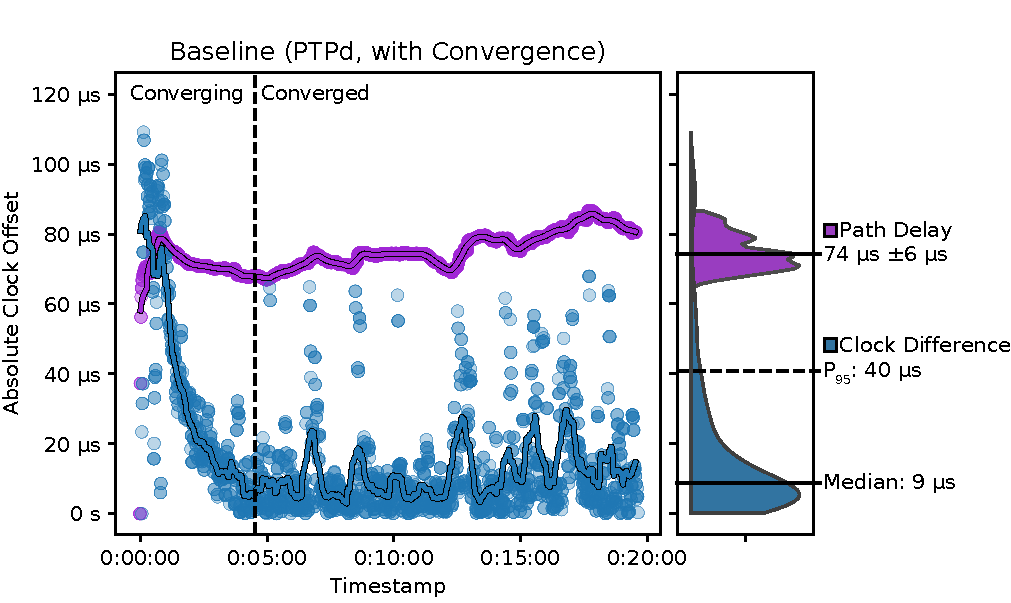
\includegraphics[width=\linewidth]{res/generated/base/rpi08-convergence_2.pdf}
    \caption{A sample run of PTPd in its default configuration (left: scattered raw signal and denoised moving average, right: kernel density estimates). Clock synchronization can follow different convergence trajectories, which needs to be accounted for when calculating statistics. Because PTP uses path delay compensation, the final clock synchronization accuracy is much better than the one-way path delay.}
    \label{fig:baseline_sample}
\end{figure}

Figure \ref{fig:baseline_sample} shows a sample run of the baseline for the PTPd vendor. In order to collect meaningful statistics, we apply some preprocessing to the collected profiles. The most important step is to remove the convergence phase (Figure \ref{fig:baseline_sample} left) from the profile to avoid it skewing the summary statistics\todo{slightly duplicated}. However, the clock travels on a different trajectory during each convergence, and each trajectory may include discontinuities, rebounds, and clock steps. To eliminate this unwanted data, we apply a heuristic to the raw clock offset (which can have positive or negative values depending on the offset direction): If the sign of the offset flips repeatedly over a specified window of time, this implies that there is no clear pattern to the measured offset that PTP can compensate for, and thus the clock offset is close to stable at its minimum value. Intuitively, this is somewhat equivalent to the average signed clock offset being zero, but note that the two are distinct for certain corner cases, as there are ways to produce an average zero clock offset that still exhibit a signal trend (which we want to avoid) and there can be large magnitude measurement outliers that cause a non-zero average clock offset while showing no trend. Empirically, we find that using the frequency of sign switches in the clock offset produces much more accurate predictions of whether a clock is synchronized than relying on average (signed) offset.

\cmpSearchVendor{\ptpKey{base/rpi-4/\vendor/pd/q50}/\ptpKey{base/rpi-4/\vendor/q50}}
From Figure \ref{fig:baseline_sample} we observe that the clock offset is much lower than the corresponding path delay, due to the path delay compensation used by PTP clients. Across the tested vendors, we observe that the median absolute clock offset is between \fRatio{\cmpMin} (\fVendor{\cmpMinArg}) and \fRatio{\cmpMax} (\fVendor{\cmpMaxArg}) smaller than the magnitude of the path delay on the Raspberry-Pi 4 cluster,%
\cmpSearchVendor{\ptpKey{base/rpi-5/\vendor/pd/q50}/\ptpKey{base/rpi-5/\vendor/q50}}%
and \fRatio[-1]{\cmpMin} (\fVendor{\cmpMinArg}) to \fRatio[-1]{\cmpMax} (\fVendor{\cmpMaxArg}) smaller on the Raspberry-Pi 5 cluster, where hardware support is available.
Logically, the absolute clock difference exhibits some amount of skew due to the fact that the value cannot be negative, and the signal can experience bursts of noise which makes determining the true clock offset more difficult. Across the profile however, the median clock offset represents the best estimate of the real clock offset, while the 95\textsuperscript{th} percentile can be used as a bound where one can be reasonably sure that the true offset is lower.

\subsection{Vendors \& Systems}

\begin{figure}
    \centering
    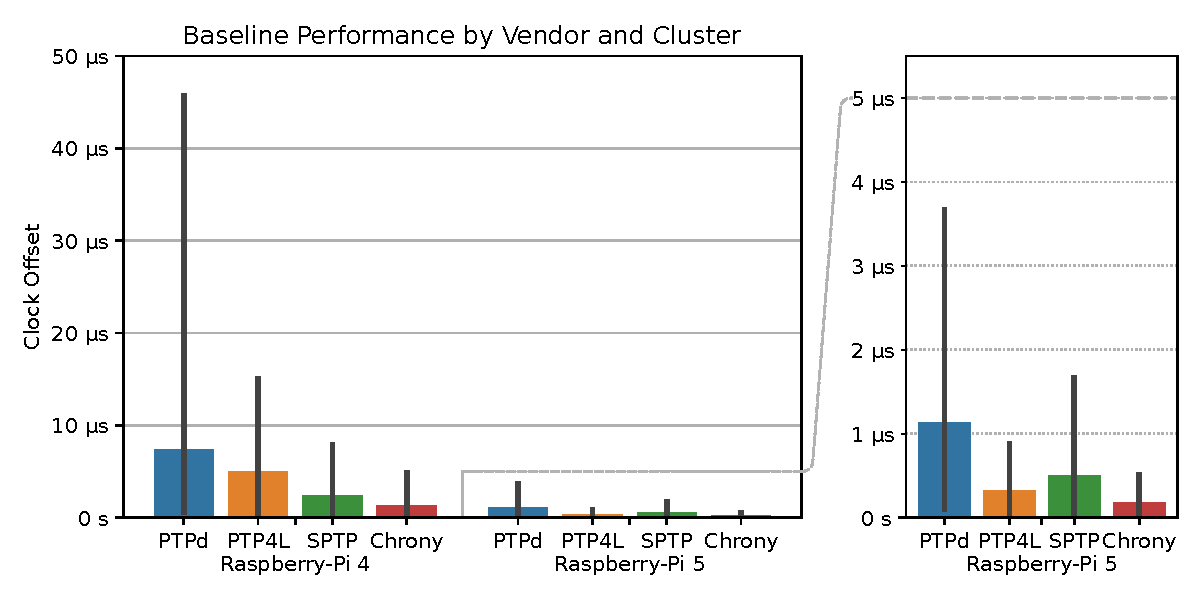
\includegraphics[width=\linewidth]{res/generated/base/vendor_comparison.pdf}
    \legend
    \caption{Median baseline performance for all vendors, across our two hardware testbeds (left) and magnified for only the Raspberry-Pi 5 cluster (right). Error bands represent the 5\textsuperscript{th} and 95\textsuperscript{th} percentiles, respectively.}
    \label{fig:baseline}
\end{figure}

\begin{table}
\centering
\caption{Baseline Values by Vendor and System}

    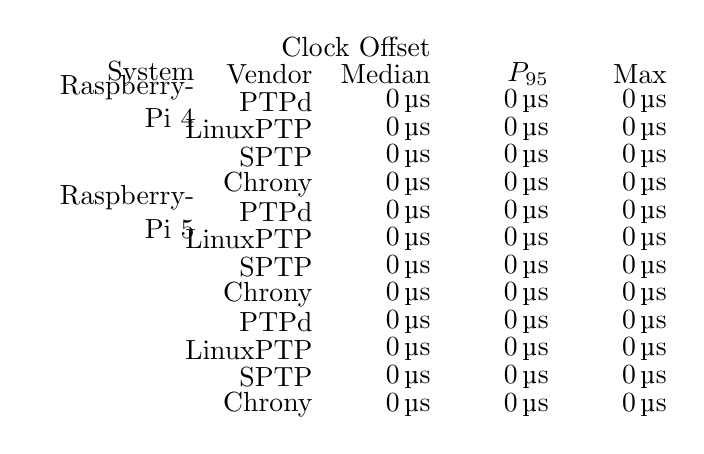
\begin{tikzpicture}[start chain=rows going below, on grid, node distance=0.35cm and 1.5cm, text width=2cm, align=right]
        \node[on chain=rows] {};
        \begin{scope}[start branch=row going right]
            \node[on chain] {};
            \node[on chain] {Clock Offset};
%            \node[on chain] {Clock Offset};
        \end{scope}

        \node[on chain=rows] {System};
        \begin{scope}[start branch=row going right]
            \node[on chain] {Vendor};
            \node[on chain] {Median};
            \node[on chain] {$P_{95}$};
            \node[on chain] {Max};
        \end{scope}

            \foreach \system in {rpi-4,rpi-5,petalinux}{
                \foreach  \vendor  in {ptpd,linuxptp,sptp,chrony}{
                    \node[on chain=rows] {\strcmpfullexpand{\vendor}{ptpd}{\fCluster{\system}}{}};

                    \begin{scope}[start branch=row going right]
                    \node[on chain] {\fVendor{\vendor}};
                    \node[on chain] {\fTimeKey[1]{base/\system/\vendor/q50}};
                    \node[on chain] {\fTimeKey{base/\system/\vendor/q95}};
                    \node[on chain] {\fTimeKey{base/\system/\vendor/q100}};
                    \end{scope}
                }
            }
    \end{tikzpicture}
    \label{tbl:baseline}
\end{table}

\cmpSearchVendor{\ptpKey{base/rpi-5/\vendor/q50}}
\cmpSave{base/rpi-5}
\cmpSearchVendor{\ptpKey{base/rpi-4/\vendor/q50}}
\cmpSave{base/rpi-4}

% Best and worst vendors are the same
\assert{\ptpKey{cmp/base/rpi-4/minarg}}{\ptpKey{cmp/base/rpi-5/minarg}}
\assert{\ptpKey{cmp/base/rpi-4/maxarg}}{\ptpKey{cmp/base/rpi-5/maxarg}}


A logical first step is comparing each vendor's baseline across the systems. Figure~\ref{fig:baseline} shows the four vendors on the Raspberry-Pi 4 and Raspberry-Pi 5 clusters, with the precise values available in Table~\ref{tbl:baseline}. We observe that \fVendor{\cmpMaxArg} has the worst synchronization offset on both systems, with a median clock offset of \fTime[1]{\cmpMax} on the Raspberry-Pi 4 and \fTimeKey[1]{cmp/base/rpi-5/max} on the Raspberry-Pi 5.
\fVendor{\cmpMinArg}, on the other hand, has the best performance on both systems, with the clock offset estimate at just \fTime[1]{\cmpMin} and \fTimeKey[1]{cmp/base/rpi-5/min}, respectively.
\assert{\cmpMinArg}{chrony}%
That a regular NTP client can outperform all of our PTP clients might come as a surprise, with PTP being engineered specifically for precision, but Chrony is very much state-of-the-art and can take advantage of the same hardware acceleration that our PTP clients can while providing a lot more features\todo{this claim might need to be backed up}.

\cmpSearchVendor{\ptpKey{base/rpi-4/\vendor/q50}/\ptpKey{base/rpi-5/\vendor/q50}}

The most noticeable effect on the synchronization quality is the choice of hardware, which is expected since the Raspberry-Pi 5 offers hardware timestamping while the Raspberry-Pi 4 does not. The newer hardware's performance advantage ranges from \fRatio{\cmpMin} for \fVendor{\cmpMinArg} to \fRatio{\cmpMax} for \fVendor{\cmpMaxArg}. Curiously, although PTPd does not support hardware timestamping and thus cannot use hardware capabilities, it still offers around \fPercentage{\ptpKey{cmp/base/rpi-5/min}/\ptpKey{base/rpi-5/ptpd/q50}} of the performance of the top contender \fVendor{\ptpKey{cmp/base/rpi-5/minarg}}. While the difference is significant, it is not orders of magnitude better than the software-only implementation, showing that hardware timestamps alone are not a cure-all solution to clock-synchronization and cannot eliminate timing variations entirely.

%\todo{
%Advantages: \foreach \vendor in {ptpd,linuxptp,sptp,chrony}{\fRatio{\ptpKey{base/rpi-4/\vendor/q50}/\ptpKey{base/rpi-5/\vendor/q50}} }
%}

\cmpSearchVendor{\ptpKey{base/rpi-4/\vendor/q95}/\ptpKey{base/rpi-4/\vendor/q50}}%
Another aspect to notice is the difference between the median clock offset and the 95\textsuperscript{th} percentile. Without hardware support, this difference can be rather large and has a high spread (between \fRatio{\cmpMin} for the most stable vendor \fVendor{\cmpMinArg} and \fRatio{\cmpMax} for the least stable vendor \fVendor{\cmpMaxArg}),
whereas the magnitude is smaller when hardware support is offered on the Raspberry-Pi %
\cmpSearchVendor{\ptpKey{base/rpi-5/\vendor/q95}/\ptpKey{base/rpi-5/\vendor/q50}}%
(\fRatio[1]{\cmpMin} \fVendor{\cmpMinArg} -- \fRatio[1]{\cmpMax} \fVendor{\cmpMaxArg}).
This means that not only is the average performance improved, but the magnitude of outliers is reduced, which is especially important when considering the dependability aspect. For applications that need to rely on timing sources, this shows that hardware acceleration can make a significant impact, but of course this comes with the price tag associated with a more capable network interface.

\subsection{Reproducibility}

% Ordering: Requires ptpKeyPrefix to be intact
\begin{figure}
    \centering
    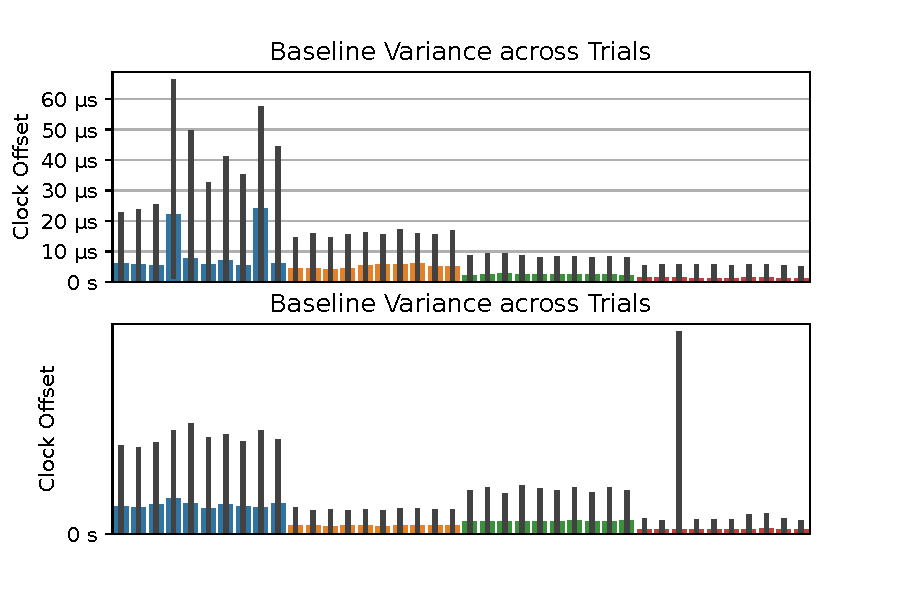
\includegraphics[width=\linewidth]{res/generated/base/key_metric_variance_compare_pi.pdf}
    \legend
    \caption{Validating the baseline results by repeatedly measuring the baseline for both vendors on the Raspberry Pi 4 system. Top: The median absolute clock offset for each run, with error bars reaching from quantiles 0.05 to 0.95. Bottom: The same for the estimated path delay.}
    \label{fig:baseline_reproducibility}
\end{figure}


{
\pgfkeys{
    /reproducibility/rpi-4/.cd,
    ptpd/min/.initial={0.000005329},
    ptpd/median/.initial={0.000005976},
    ptpd/max/.initial={0.000024082},
    linuxptp/min/.initial={0.0000041995},
    linuxptp/median/.initial={0.0000049845},
    linuxptp/max/.initial={0.0000059645},
    sptp/min/.initial={0.000002234},
    sptp/median/.initial={0.000002448},
    sptp/max/.initial={0.0000027660000000000003},
    chrony/min/.initial={0.00000125},
    chrony/median/.initial={0.0000012990000000000002},
    chrony/max/.initial={0.0000014060000000000002},
}
\renewcommand{\ptpKeyPrefix}{/reproducibility/rpi-4}



\newcommand{\numBaselineMeasurements}{10}
\newcommand{\baselineMinutesRuntime}{\numBaselineMeasurements*4*2*20}

The next question to be answered is how reproducible the measurement results are. Previously, all baseline results were aggregated into a single metric, but in reality the baseline consists of a number of independent measurements, which are interleaved for better compensation of noise that may be introduced through mechanisms outside our control. We repeated the measurement of the baseline observations ten times for each vendor on each hardware platform (totaling in around \fpeval{round(\baselineMinutesRuntime/60)} hours of runtime and \fpeval{round(\baselineMinutesRuntime*60)} samples collected) and aggregate them. Between each measurement run, the entire cluster is restarted to ensure that no state is carried over, which would harm the independence of observations. Otherwise, the setup is left untouched, so the only differences occur in the internal state of PTP.

\cmpSearchVendor{\ptpKey{\vendor/max}/\ptpKey{\vendor/min}}

Figure \ref{fig:baseline_reproducibility}\todo{Graphic not super useful, increase information density.} shows the results for two vendors, PTPd and LinuxPTP. We observe that LinuxPTP produces significantly more stable results for both the clock offset estimation and the path delay, while PTPd shows more variance in median and 95-th quantile observed clock offset across independent measurements. Additionally PTPd's path delay estimation shows a higher variance. A simple restart of the PTPd client can suddenly cause the median latency to jump from \fTimeKey{ptpd/min} up to \fTimeKey{ptpd/max}, which corresponds to an increase of \fRelative[-1]{\ptpKey{ptpd/max}/\ptpKey{ptpd/min}} not only momentarily, but throughout an entire run of 20 minutes.
%This already comes uncomfortably close to our safety factor of \safetyMargin, and we have not even started stressing the system yet.
Fortunately, LinuxPTP produces a lot more stable results, with a smaller range of \fTimeKey{linuxptp/min} and \fTimeKey{linuxptp/max} between the best observed run and the worst observed run, corresponding to just \fRelative{\ptpKey{linuxptp/max}/\ptpKey{linuxptp/min}} difference. The best vendor in this regard is \fVendor{\cmpMinArg} (not shown), with a range of just \fRelative{\cmpMin}, while the worst performance is observed with the aforementioned \fVendor{\cmpMaxArg}.
%
% Assert last sentence
\assert{\cmpMaxArg}{ptpd}
%
Needless to say, a vendor that cannot deliver stable timing guarantees is risky to deploy in a production environment that needs to rely upon the time source functioning. In the upcoming sections, we will examine whether PTP clients can be made resilient against potential external and internal influences.

}

\section{Resource Contention}

One aspect that influences how reliable PTP can operate is the outside interference originating from resource sharing. Through our research, we examined a range of shared resources that might impact synchronization accuracy and therefore need to be carefully managed so that PTP can provide synchronization even in the presence of stress. Unsurprisingly, the key resource tends to be the network.

\subsection{Network Contention}
\begin{figure}
    \centering
    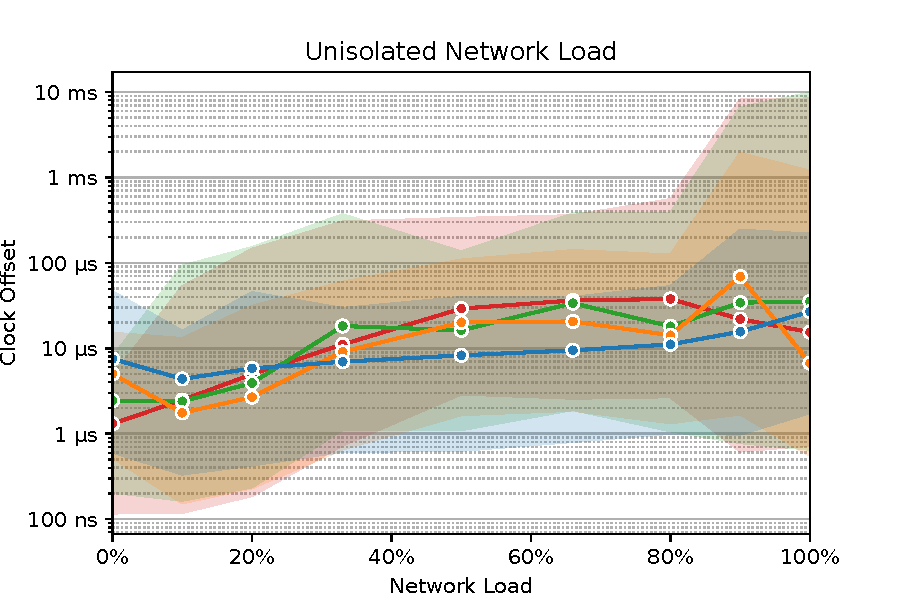
\includegraphics[width=\linewidth]{res/generated/net_unprioritized_trend_rpi-4.pdf}
    \legend
    \caption{Clock synchronization accuracy at different levels of network load. All vendors experience degradation at higher network loads, though the degree to which they are affected differs. Apart from a change in median clock offset, the 95\textsuperscript{th} percentile is heavily affected, signaling larger and more frequent outliers.}
    \label{fig:network_load}
\end{figure}

\cmpSearchVendor{\ptpKey{load/net_unprioritized/load_100/rpi-4/\vendor/q50}/\ptpKey{base/rpi-4/\vendor/q50}}

Like stated previously, the synchronization accuracy principally depends on the magnitude and the variation of the path delay. Intuition therefore suggests that the more network load is present, the more PTP will struggle to measure the clock offset consistently due to increased queuing in software and hardware causing delay and delay variation in delivery. We simulate network load artificially using iPerf, a traffic generator that allows us to target predefined data rates. By default, when a PTP vendor is installed on a target system and run, there are no special precautions in place to guard against contention, so a decrease in accuracy as the network load increases is exactly what we observe (Figure \ref{fig:network_load}). Interestingly, the vendor with the smallest increase in clock offset is \fVendor{\cmpMinArg}, with an increase of just \fRatio[1]{\cmpMin} (\fTimeKey{base/rpi-4/\cmpMinArg/q50} -- \fTimeKey{load/net_unprioritized/load_100/rpi-4/\cmpMinArg/q50}) from no network load to 100\% network load. On the other hand, \fVendor{\cmpMaxArg} has a much higher ratio of \fRatio{\cmpMax} (\fTimeKey{base/rpi-4/\cmpMaxArg/q50} -- \fTimeKey{load/net_unprioritized/load_100/rpi-4/\cmpMaxArg/q50}), which can only be partially attributed to the fact that \fVendor{\cmpMaxArg} has a smaller baseline value.
% Assert SPTP is worst
\assert{\cmpMaxArg}{sptp}%
SPTP is the only vendor that relies solely on unicast message exchange (a design choice by Meta), whether this is why SPTP appears to be more susceptible to contention is subject to further investigation.%
%
% 95-th percentiles
\cmpSearchVendor{\ptpKey{load/net_unprioritized/load_100/rpi-4/\vendor/q95}/\ptpKey{base/rpi-4/\vendor/q95}}%
\cmpSave{net_load_vs_baseline} % Used in conclusion
The 95\textsuperscript{th} percentiles reflect the behavior of the outliers, and here we can observe even larger ranges, with \fVendor{\cmpMaxArg} now showing a ratio of \fRatio[-1]{\cmpMax} (\fTimeKey{base/rpi-4/\cmpMaxArg/q95} -- \fTimeKey[-1]{load/net_unprioritized/load_100/rpi-4/\cmpMaxArg/q95}). This is clearly above and beyond even very generous safety margins, so we need to examine how the effect of network load can be mitigated.

 Note that under network load PTP sometimes fails to even synchronize at all, when it gets stuck in an infinite loop running into transmission timeouts and thus switching between ``state init'' and ``state faulty''. In this case the timing system breaks entirely, and no synchronization can be established. These measurements have been excluded from the shown data, but we encountered them rather frequently at high load levels. Preventing this is paramount, as having no synchronization and potentially not even being aware of it is a lot worse than having a bad quality signal.

\begin{figure}
    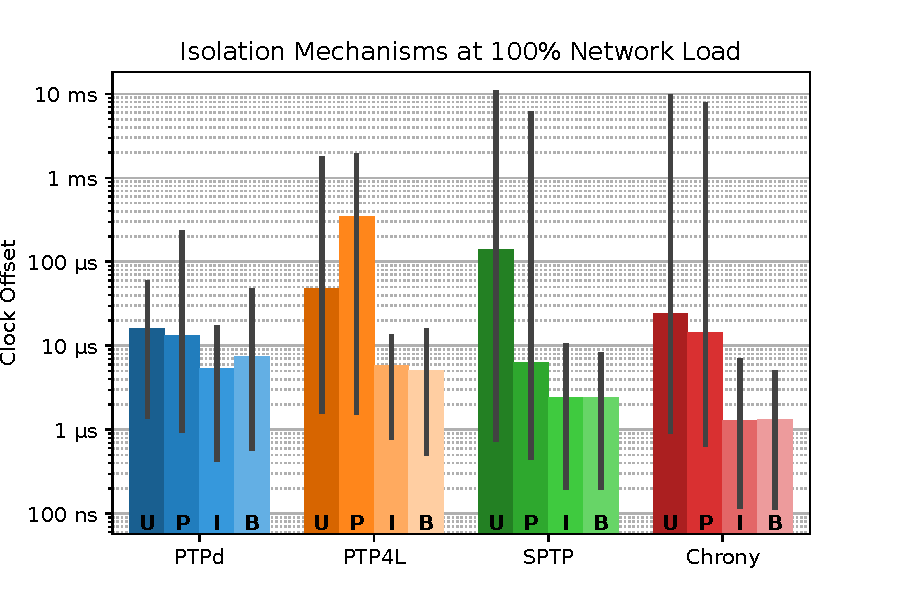
\includegraphics[width=\linewidth]{res/generated/net_isolation_comparison.pdf}
    \begin{center}
    \vspace{-0.5cm}
    \sffamily\scriptsize \textbf{U}: Unprioritized \quad\textbf{P}: Prioritized \quad\textbf{I}: Isolated \quad\textbf{B}: Baseline
    \end{center}
    \begin{center}
    \legend
    \end{center}
    \caption{Different possibilities of isolating the network load, compared to the baseline with no load. Both prioritization and physical isolation can often improve performance over the unprioritized default, however only isolation can match the performance of the baseline without resource contention.}
    \label{fig:net_isolation_comparison}
\end{figure}

Depending on the possibility of dedicating exclusive resources to PTP, two principle solutions are viable: a software/hardware prioritization of traffic to reduce interference of lower priority traffic and providing a dedicated network interface for physical isolation. While the latter might seem like an expensive proposition and could therefore be less suited for embedded solutions, other use cases like industrial or datacenter settings will often already provide a second management interface separate from the application's network. On our Raspberry-Pis, we emulate this by configuring the routing table so only PTP traffic can use the wired interface, with other traffic being relegated to the wireless interface. Figure~\ref{fig:net_isolation_comparison} shows these possibilities, with the default unisolated case on the left and the baseline on the very right.%
\cmpSearchVendor{\ptpKey{load/net_isolated/load_100/rpi-4/\vendor/q50}/\ptpKey{base/rpi-4/\vendor/q50}}%
%Worst: \fRatio[1]{\cmpMax} @ \cmpMaxArg{} and \fRatio[1]{\cmpMin} @ \cmpMinArg
\assertRange{\cmpMax}{1.0}{1.5}%
\assertRange{\cmpMin}{0.6}{1.0}%
Conforming to expectations, a physical isolation of PTP traffic can entirely mitigate the adverse effects of network load, with results sometimes even outperforming the baseline slightly (\fVendor{\cmpMinArg}: \fRelative{\cmpMin}, \fVendor{\cmpMaxArg}: \fRelative{\cmpMax}).
Theoretically, the only interference that could traverse the isolation barrier is latency caused by cross-talk on the software network stack, which does not appear to be an issue here.

The prioritization-based solution, however, cannot quite achieve the same level of performance on our testbed. Prioritization is achieved through differentiated services (via the Differentiated Services Code Point, DSCP), and requires prioritization support on every networking software and hardware component on the critical path to perform optimally. While our switch and operating system claim to support the technology, this does not appear to be sufficient for complete traffic segregation.
\cmpSearchVendor{\ptpKey{load/net_unprioritized/load_100/rpi-4/\vendor/q50}/\ptpKey{load/net_prioritized/load_100/rpi-4/\vendor/q50}}
Compared to no traffic prioritization, activating DSCP results in performance improvements up to \fRatio{\cmpMax} for \fVendor{\cmpMaxArg}.
However, one anomaly exists, which is \fVendor{\cmpMinArg}, where the median vendor performance actually decreases by \fRatio{1/\cmpMin}, while the 5\textsuperscript{th} and 95\textsuperscript{th} percentiles remain the within 3$\times$ the baseline.
\assertRange{\cmpMin}{0.01}{0.1}%
\assertRange{\ptpKey{load/net_unprioritized/load_100/rpi-4/linuxptp/q95}/\ptpKey{load/net_prioritized/load_100/rpi-4/linuxptp/q95}}{0.3}{1.0}%
\assertRange{\ptpKey{load/net_unprioritized/load_100/rpi-4/linuxptp/q5}/\ptpKey{load/net_prioritized/load_100/rpi-4/linuxptp/q5}}{0.3}{1.0}%
%
\newcommand{\numTrials}{min(\ptpKey{load/net_unprioritized/load_100/rpi-4/linuxptp/count}, \ptpKey{load/net_prioritized/load_100/rpi-4/linuxptp/count})}%
We have examined the affected profiles in more detail and can confirm that this effect is visible on all \fNum{\numTrials} trials encompassing approximately \fNum{\numTrials * 20 * 60} samples, so while we are confident of the validity of the observation, the reason why it occurs is currently unknown.

\todo{Perhaps recommendations}

\subsection{Other shared resources}

\cmpSearchVendor{\ptpKey{load/cpu_unprioritized/load_100/rpi-4/\vendor/q50}/\ptpKey{base/rpi-4/\vendor/q50}}
\cmpSave{q50}
\cmpSearchVendor{\ptpKey{load/cpu_unprioritized/load_100/rpi-4/\vendor/q95}/\ptpKey{base/rpi-4/\vendor/q95}}
\cmpSave{q95}

We have  further examined the effect of contention on other shared resources, and fortunately none of them cause synchronization quality degradation at the level that network congestion does.
An educated guess for the next most important shared resource could be CPU, as difficulties to get scheduled timely intuitively could cause delays in packet processing.
However, our data shows this is not the case on the Raspberry-Pi 4, as CPU contention only causes a maximum observed median degradation of just \cmpLoad{q50}\fRelative{\cmpMax} (\fVendor{\cmpMaxArg}) and \cmpLoad{q95}\fRelative{\cmpMax} at the 95\textsuperscript{th} percentile on the Raspberry-Pi 4, which is small enough not to make a practical difference.
\assert{\cmpMaxArg}{chrony}
This is likely due to the fact that PTP clients do not consume much processing time, which means they can easily get scheduled on Linux's Completely Fair Scheduler (CFS) even when idle computing time is scarce.
Interestingly, CPU load can actually boost performance relative to the baseline for \cmpLoad{q50}\fVendor{\cmpMinArg} by around \fRelativeInverted{\cmpMin} for the median value and \cmpLoad{q95}\fRelativeInverted{\cmpMin} for the 95\textsuperscript{th} percentile (\ptpKey{load/cpu_unprioritized/load_100/rpi-4/\cmpMinArg/count} trials, $\sim$\fNum{\ptpKey{load/cpu_unprioritized/load_100/rpi-4/\cmpMinArg/count} * 20 * 60} samples).
\cmpLoad{q50}\assertRange{\cmpMin}{0}{0.8}% Anything below 1 is decrease
\cmpLoad{q95}\assertRange{\cmpMin}{0}{0.8}% Anything below 1 is decrease
\assert{\ptpKey{cmp/q50/minarg}}{\ptpKey{cmp/q95/minarg}}%
%
We assume that this benefit originates from less scheduling variance when the processor is kept busy due to less power saving.
\cmpSearch{\vendor}{chrony,linuxptp}{\ptpKey{load/cpu_unprioritized/load_100/rpi-5/\vendor/q50}/\ptpKey{base/rpi-5/\vendor/q50}}%
\assertRange{\cmpMax}{1.0}{1.2}%
On the Raspberry-Pi 5, things look a little different. While Chrony and LinuxPTP are mostly unaffected (up to just \fRelative{\cmpMax} overhead),
\cmpSearch{\vendor}{sptp,ptpd}{\ptpKey{load/cpu_unprioritized/load_100/rpi-5/\vendor/q50}/\ptpKey{base/rpi-5/\vendor/q50}}%
\assertRange{\cmpMin}{1.6}{3.0}%
SPTP and PTPd have a more noticeable degradation in synchronization performance of up to \fRatio[1]{\cmpMax}, which is however not nearly as critical as the previous degradation through network congestion.

\cmpSearchVendorCluster{\cmpRatioVendorClusterVsBaseline{load/aux_cache/load_100}}%
\cmpSave{cache}%
The third principal hardware component where contention can occur is the memory hierarchy. Generally, PTP does not require a huge amount of resources, and we can see this reflected in the sensitivities against cache contention (between \fRatio[1]{\cmpMin} with \fVendorCluster{\cmpMaxArg} and \fRatio[1]{\cmpMax} with \fVendorCluster{\cmpMaxArg})\todo{Await results},%
\cmpSearchVendorCluster{\cmpRatioVendorClusterVsBaseline{load/aux_memory/load_100}}%
\cmpSave{memory}%
which is slightly higher than what we observe for memory bandwidth contention (up to \fRatio{\cmpMax} with \fVendorCluster{\cmpMaxArg}).
\assertRange{\cmpKey{memory}{max}}{0}{\cmpKey{cache}{max}*0.75}%
In the end, both memory bandwidth contention and cache contention turn out to be more important than CPU contention.%
% q50 is cpu_unprioritized, ugh.
\assertRange{\cmpKey{q50}{max}}{0}{\cmpKey{memory}{max}*0.75}%

We have put the PTP clients through further stress tests (leveraging the capabilities provided by Stress-NG) and observe the following:%
\begin{itemize}
    \item Stressing time-related kernel features such as timers or alarms do not impact PTP performance significantly (with a maximum deviation from the baseline of under 50\%).
    \cmpSearchVendorCluster{\cmpRatioVendorClusterVsBaseline{load/aux_timer/load_100}}%
    \assertRange{\cmpMax}{0.5}{1.5}%
    \cmpSearchVendorCluster{\cmpRatioVendorClusterVsBaseline{load/aux_alarm/load_100}}%
    \assertRange{\cmpMax}{0.5}{1.5}%
    \item Installing cyclic tasks with a deadline in the schedule (\texttt{SCHED\_DEADLINE}), which might cause PTP to get deferred when a real-time task needs to be scheduled, also do not cause significant adverse effects. This is good news as applications that require precise notions of time will often also be time-critical, and thus they usually use a real-time scheduling policy. However, note that things will likely start to fall apart when real-time tasks hog almost all available compute, as this will make it difficult for PTP to get scheduled at all unless it is promoted to a corresponding scheduling policy itself (which is not the case for the default profile).
    \cmpSearchVendorCluster{\cmpRatioVendorClusterVsBaseline{load/aux_cyclic/load_100}}%
    \assertRange{\cmpMax}{0.5}{1.5}%
    \item Finally, all PTP implementations also show good resilience against excessive context switching, which places stress on multiple software and hardware components simultaneously.
    \cmpSearchVendorCluster{\cmpRatioVendorClusterVsBaseline{load/aux_switch/load_100}}%
    \assertRange{\cmpMax}{0.5}{1.5}%
\end{itemize}

While resource contention, especially network congestion, can lead to degradation of clock synchronization performance, it is not the sole reason that the time synchronization system may fail.

%Interestingly, some level of load can actually boost performance relative to the baseline (we observed this on both the CPU and the network).
%We assume this occurs due to the hardware switching less into power saving states when more load is present, which may actually cause packets to be delivered faster.

\section{Fault Tolerance}
\newcommand{\faultLength}{30 seconds}

\begin{figure}
    \begin{center}
    \begin{tikzpicture}[component/.style={draw}, node distance=0.5cm]
        \node[component, ] (master) {\faBug{} \faBolt{} Master};
        \node[component, right=of master] (network) {\faBolt{} Network};
        \node[component, right=of network] (primary-slave) {\faBug{} \faBolt{} Primary Slave};
        \node[component, below=0.25cm of primary-slave] (secondary-slave) {Secondary Slave*};

        \draw[-] (master) -- (network);
        \draw[-] (network) -- (primary-slave);
        \draw[-] (network) |- (secondary-slave);
    \end{tikzpicture}
    \end{center}

    \scriptsize *: For certain outlined scenarios, the secondary slave gets promoted to a failover master when the master fails.

    \caption{
        Simple fault-setup consisting of three clients, where potential software (\faBug{}) or hardware (\faBolt{}) faults may occur. Since we exclude compound failures, only one fault can occur simultaneously, so no faults are triggered in the secondary slave.
    }
    \label{fig:fault_architecture}
\end{figure}

Apart from resource contention, faults are another key threat to the functioning of the timing system. We examine faults originating from three distinct causes: a fault in the network, a fault in the software, and a fault in the hardware. The software/hardware faults can either occur on a PTP slave, in which case they are less critical as the expectation is that the failure will be relatively contained within a single node, or on the PTP master, in which case they are more critical as the failure could propagate across the PTP domain. In high-reliability deployments, there will typically be a failover master to take over upon a fault in the master, so we examine that scenario too. Figure~\ref{fig:fault_architecture} shows an overview of the locations and types of faults that may occur. We emulate software faults by hard terminating the PTP client in software -- in reality such a fault might come from within the client due to e.g. a bug, or from an external source (e.g. a process kill during an out-of-memory situation). We produce simulated hardware faults using our programmable power delivery unit, which is equivalent to a loss-of-power scenario, but real-life production hardware faults and system hang-ups could also come from other component failures.

\subsection{Software Fault -- Slave}

\cmpSearchVendor{\ptpKey{fault/software/slave/rpi-4/\vendor/count}}
\xdef\bSoftwareFaultNumProfiles{\cmpMax}
\newcommand{\maxClockSlew}{(0.05/100)}
\newcommand{\windowOfUncertaintyOneMinute}{(60*(\maxClockSlew))}

\begin{figure}
    \centering
    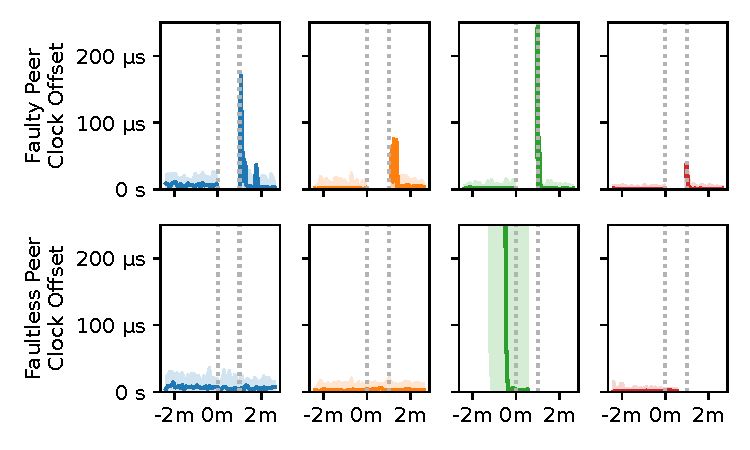
\includegraphics[width=\linewidth]{res/generated/fault/software/slave_rpi-4_peer_comparison.pdf}
    \legend
    \caption{Faults induced by a software crash on Raspberry-Pi 4, with a faulty client (shown on the left) and a second client as a control (right). Just after the fault, an increased offset can be observed as PTP tries to resynchronize the clock. Since these offsets occur randomly, we superimpose \fNum{\bSoftwareFaultNumProfiles} trials for each vendor so that the worst case can be seen.}
    \label{fig:software_fault}
\end{figure}

The simplest possible fault is a PTP client crashing, because the only state that is lost is the state within the PTP slave client application (such as the state of the servo disciplining the clock). While the PTP application is down, the clock will continue to drift at the real clock drift rate minus the compensation rate that was last set by the PTP application. If the synchronization before the crash was stable, this observed drift rate is expected to be comparatively low. However, in the worst case when the clock slew is at the maximum rate (as will often be the case in the early stages of convergence), the software-driven drift can be up to 0.05\%~\cite{adjtimex}, which can cause a software-induced drift of \fTime{0.05/100} per second of downtime, or \fTimeMS{\windowOfUncertaintyOneMinute} per minute. We wish to determine empirically how big the offset is from a software fault when the clock is stable.

\cmpSearchVendor{\ptpKey{fault/software/slave/rpi-4/\vendor/fault/post_max/max}}

From the results (Figure~\ref{fig:software_fault} left), we can determine that the maximum observed offset after a 1-minute software fault among \fNum{\bSoftwareFaultNumProfiles}\todo{import more trials} trials is \fTime{\cmpMax} for \fVendor{\cmpMaxArg}, which is around \fRatio{\cmpMax/\ptpKey{base/rpi-4/\cmpMaxArg/q50}} worse than the median baseline performance. While this drift is definitely noticeable, it is fortunately not even close to the theoretical worst-case window of uncertainty of \fTimeMS{\windowOfUncertaintyOneMinute}, representing just \fPercentage[2]{\cmpMax/\windowOfUncertaintyOneMinute} of the maximum software induced drift. We also observe that it is possible to get lucky: in some trials there is very little observed offset despite a full minute of downtime (just \fTime{\cmpMin} with \fVendor{\cmpMinArg}). In any case, all PTP implementations can quickly reconverge on the clock signal within a few seconds of restarting. Due to a quirk in how the PTP protocol works (slaves request synchronization signal leases from the master with a predetermined expiry), the master node will keep sending synchronization messages to the dead peer, which combined with the second lease that is issued when the PTP slave is restarted can help the peer synchronize quicker due to the higher influx of synchronization messages (this is sometimes referred to as an abandoned sync~\cite{sptp}).

In high reliability deployments, replication is frequently applied to increase dependability. However, in order for replication to be useful, we need to ensure that a failure can be contained to the node of origin. In terms of PTP, this means that the fault on one slave should not affect the quality of synchronization of the other slave. To verify that this is the case, we attached a second control node to the same master (Figure~\ref{fig:software_fault} right\todo{improve graphic}), which shows us that there is no meaningful degradation of the performance of other nodes.

One important caveat is to be noted for PTPd: when multiple software faults start occurring (not necessarily in close proximity to each other), problems can start propagating. On our test systems, we observe that upon exactly the third software fault, PTPd will cause the network interface to fail. In fact, no amount of manually bringing the network down and back up or reloading the network interface driver can solve this problem, up until the system is restarted by hand. This is especially critical as it implies that not only will the timing system fail, but it will simultaneously bring down any applications that need to communicate over the interface as well. Ironically, in this case, rather than support the deployment high-reliability distributed systems, PTPd will actually harm said reliability. We thus advise caution when deploying PTPd or any of its derivatives that may contain the same bug.

\subsection{Hardware Fault -- Slave}
\cmpSearchVendor{\ptpKey{fault/hardware/slave/rpi-4/\vendor/fault/post_max/max}}
\xdef\maxPiFour{\cmpMax}
\cmpSave{hw_slave_rpi-4}

\cmpSearchVendor{\ptpKey{fault/hardware/slave/rpi-5/\vendor/fault/post_max/max}}
\xdef\maxPiFive{\cmpMax}
\cmpSave{hw_slave_rpi-5}


\begin{figure}
    \centering
    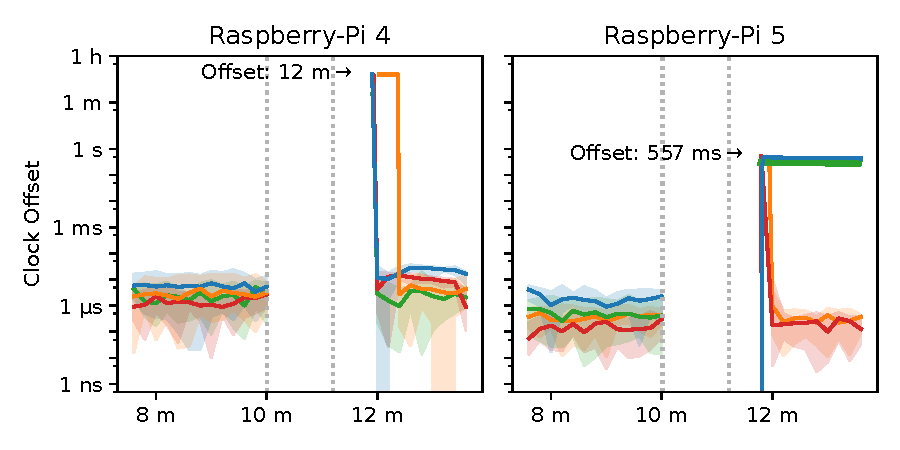
\includegraphics[width=\linewidth]{res/generated/fault/hardware/slave_cluster_comparison.pdf}
    \legend
    \caption{A hardware fault on the slave of the Raspberry-Pi 4 cluster (left) and the Raspberry-Pi 5 cluster (right). Both slaves need to fully resynchronize after rebooting, but the Raspberry-Pi 5 has an advantage due to its hardware clock.}
    \label{fig:hardware_fault_slave}
\end{figure}

A slightly more difficult scenario is a hardware fault on the slave, as not only will the internal PTP state be lost, but also the kernel state containing the current system time and the clock drift. This implies that PTP will need to fully reconverge, using the standard step-and-slew approach seen in the baseline. Because the Raspberry-Pi 4 (Figure~\ref{fig:hardware_fault_slave} left) does not contain a real-time clock to preserve the system time across reboots, after a reboot a node will have a system time equal the last time that the time was persisted to disk if fake-hwclock~\cite{fake-hwclock-manpage} is active or a default value (e.g. the epoch in 1970) if fake-hwclock is not active. On our system (Raspbian, which bases on Debian), fake-hwclock is configured, so we observe a temporary deviation of just \cmpLoad{hw_slave_rpi-4}\fTimeMin{\cmpMax} (on \fVendor{\cmpMaxArg}). To fix the large offset, PTP needs to step the clock (breaking invariant I2) and then takes some minutes to reconverge on the previous level of accuracy (in the case of PTPd, the other vendors are generally faster). On the other hand, the Raspberry-Pi 5 can maintain the current time using the hardware clock while it is not running\todo{Fault not visible on RPI-5 chart}. While the RTC generally has lower resolution than the internal oscillator (a common resolution is 1/32768), it generally has good long-term stability\todo{cite}. This advantage shows itself in the observed maximum offset, which is a comparatively tiny \cmpLoad{hw_slave_rpi-5}\fTime{\cmpMax} (\fVendor{\cmpMaxArg}), a full \fNum{ln(\maxPiFour/\maxPiFive)/ln(10)} orders of magnitude smaller that can easily be compensated by clock slew only. A fault on a system without a hardware clock will thus cause an application to encounter large inconsistencies in timing in a place where it might not expect it (right in the middle of a run), while a simple RTC can mitigate this problem entirely. For deployments that are stuck on systems where an RTC is not viable (e.g. due to cost reasons), it is recommended to configure a delay for the application relaunch to allow PTP to resynchronize first.

\subsection{Hardware Fault -- Master}

\begin{figure}
    \centering
    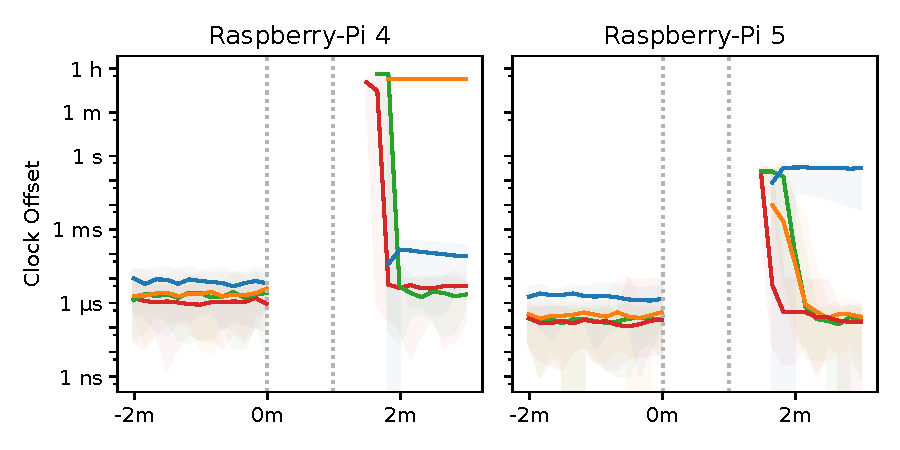
\includegraphics[width=\linewidth]{res/generated/fault/hardware/master_cluster_comparison.pdf}
    \legend
    \caption{A hardware fault on the master of the Raspberry-Pi 4 cluster (left) and the Raspberry-Pi 5 cluster (right). Slaves cannot compensate for unexpected changes in the announced time without correct configuration, so large clock offsets may be present practically indefinitely.}
    \label{fig:hardware_fault_master}
\end{figure}


PTP slaves are not the only type of node that can fail, the PTP master can just as well be affected by a disruption. Of all the scenarios, this is the most difficult one, as a failure will cause all slave nodes to become desynchronized. A failure on the master will inevitably also lead to hiccups on the announced time, especially in the embedded scenario where no external clock source for ground truth is available. On the Raspberry-Pi 4 (Figure~\ref{fig:hardware_fault_master} left\todo{Fix this chart too}), we observe that when the master restarts and now has a different reference time, there is once again a large offset between the master time and the slave time. However, unlike previously, the slave nodes are now no longer able to compensate for the offset by creating a clock step and instead are stuck at an (almost) constant offset to the master node. The reason for this lies in the default configuration of the PTP clients: It is assumed that stable time needs to be served to the application, so invariants I1 and I2 may not be broken, except once at start-up time when a single clock step is permissible to avoid excessive convergence time through clock slew. Because the slaves did not restart, they are not allowed to perform a clock-step, and while they can easily observe the difference they are stuck converging on it with a regular clock slew, which for the observed offset of \fTimeMin{\maxPiFour} is projected to require at least \fTimeMin[-3]{\maxPiFour/\maxClockSlew} -- clearly impractical. Moreover, while the slaves will be converging on the new master clock at close to the maximum software drift rate simultaneously, we observe that they do not stay particularly well in sync between each other while this happens because the hardware clock drift continues to differ between nodes, which means that the remaining peers can also not rely on their clocks being close to each other either. This problem of indefinite clock-slew can be avoided by reconfiguring the PTP slave to also allow subsequent clock steps (which is disabled by default for safety), but the system should be well tested for resilience as the application will have to cope with a large magnitude rewinding of the clock (this is the worst case, breaking both I1 and I2). Experimentation on the stress-test tools and other applications show that many misbehave during a clock step, so it cannot be assumed that an application is resilient simply because it uses the monotonic clock.

As already observed previously, the issue is easily mitigated by using an external clock that can maintain system time during downtime (e.g. Raspberry-Pi 5). The clock source does not need to be of particularly high quality if the goal is to only maintain sub-second synchronization accuracy. Should constraints only allow an external clock to be installed on a single node, intuition and our observations suggest that the primary target for installation should be the master node -- it can propagate its stable time source to the slaves.

\subsection{Hardware Fault -- Failover Master}

\begin{figure}
    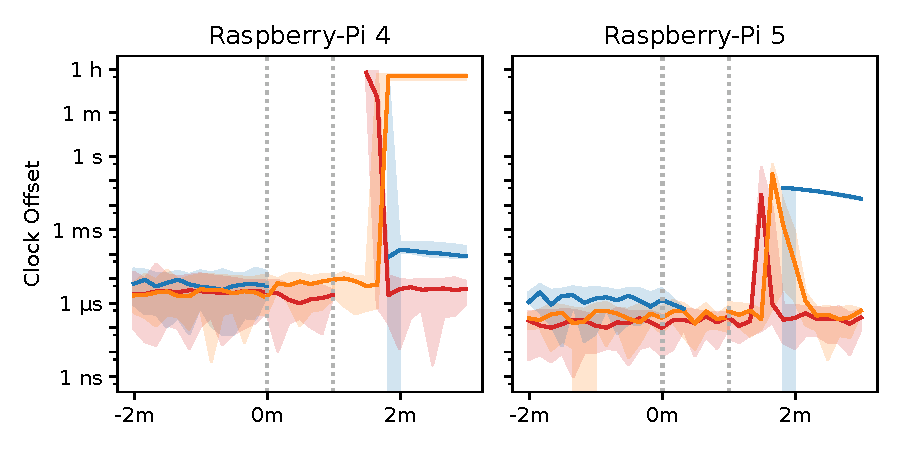
\includegraphics[width=\linewidth]{res/generated/fault/hardware/master_failover_cluster_comparison.pdf}
    \caption{Fault Tolerance with a Failover Master}
    \label{fig:failover}
\end{figure}

To increase service availability it is common to install a failover for any single point of failure in a distributed system so that the backup system can take over when the primary system fails. This is not only applicable for data-centers, but also applies to our minimal three node embedded setup, as a failover master will allow the two remaining nodes to remain synchronized with each other when the primary master fails. Fortunately, PTP was designed with this explicitly in mind so that the failover master does not necessarily require its own clock source, the failover node can automatically assume a slave state while the master is healthy (thus acquiring a clock signal consistent with the master's) and subsequently promote itself to a master when the original master is no longer healthy. Note that this setup is not supported in Meta's SPTP, as masters and slaves run different binaries and thus cannot switch roles (an external clock source would be necessary for two synchronized masters, we thus exclude SPTP from this evaluation).

We observe that the failover master can very rapidly take over the master role in the event of a failure, causing virtually no disruption in the timing service (Figure~\ref{fig:failover}\todo{data import failed}). However, the presence of a failover master cannot mitigate the problem of the master eventually restarting and disseminating a different time, which will be picked up by the failover master and the slaves, who will proceed to again get stuck in an indefinite clock slew. Due to the way the best master clock algorithm works (the same master clock will always be selected unless a configuration is changed thus shifting the prioritization), the failover master cannot re-teach the current network time to the master that has just restarted because it does not take priority over the actual master unless the master is demoted through configuration (e.g. using data from an external clock source).

\subsection{Network Fault}

Another possible root cause for a fault is the network. While a network outage is generally bad news for reliable distributed systems that need to communicate, a total network outage is ironically easier for PTP to handle than a functioning network with high levels of congestion or a contained failure within any of the nodes. Since no state is lost, the servos are kept in holdover and PTP just has to detect when the network is available again to reconverge on the common network time. The effects of this scenario are not particularly surprising, so we do not show it separately\todo{include perhaps 1 number}.


\section{Resource Consumption}
\todo{Find where to place this section.}

\begin{figure*}
\centering
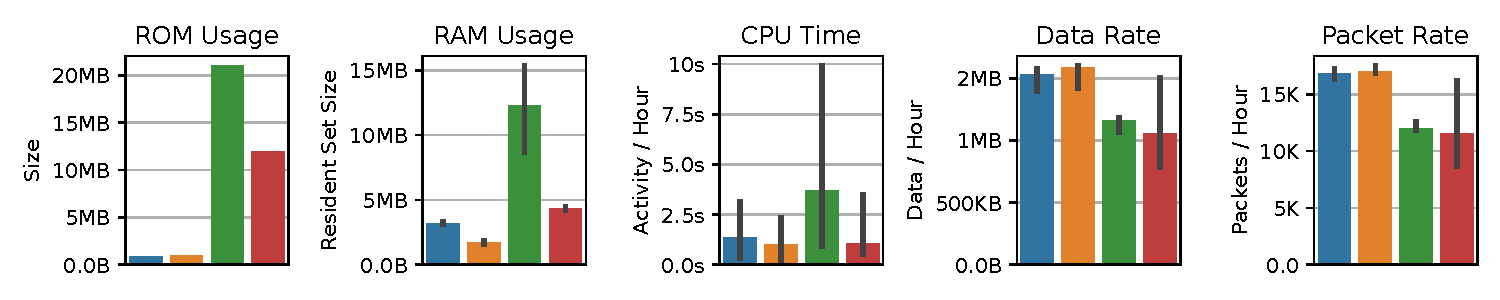
\includegraphics[width=\linewidth]{res/generated/resource_consumption/summary.pdf}
\legend
\caption{Resource consumption statistics across vendors and systems. In general, PTP systems use few onboard resources but generate more network traffic, while the evaluated NTP and SPTP implementations reduce network utilization at the cost of additional ROM and other on-board resources.}
\label{fig:resource_consumption}
\end{figure*}

Finally, embedded systems need to take particular care of the resource consumption of their applications. Since time synchronization fulfills only a supporting role in the overall deployment, it is important that it does not detract significantly from the resources available for the actual application. This is not only true for resources with a hard limit (compute, memory, etc.) but also for ``soft'' resources like power draw and heat dissipation. Especially SPTP was created with the intention of less resource consumption in mind~\cite{sptp}, so we will verify whether reality holds up to these claims.

While some PTP systems are specifically tied to Linux and thus come with the associated resource requirements, others can also be deployed in more lightweight environments. On low capability devices, ROM/flash space is generally restricted, so the footprint becomes a concern. PTPd has the comparatively lightest footprint, with executables, data and dependencies totaling at around 840\,KB after removal of pre-packaged documentation and dependencies that can reasonably be expected to already be available (e.g. lib-c). The LinuxPTP package is larger but requires fewer dependencies, thus the resulting footprint of 970\,KB is around the same. SPTP (21\,MB) and Chrony (12\,MB) are both more than an order of magnitude larger due to the integrated Go runtime and the comparatively large number of dependencies, respectively. Note that the size of SPTP could be reduced by around 40\% by only deploying the master or client executable and the Chrony footprint is significantly smaller if the larger dependencies (iproute2 + libgnutls30 + tzdata $=$ 10\,MB) are already available. In combination with an embedded Linux distribution, the more lightweight systems could reasonably be deployed on 16\,MB flash devices, although this would likely not leave sufficient headroom for the actual application -- thus 32\,MB is the more realistic lower bound for PTP deployments.

Closely tied to the storage footprint is the memory footprint. LinuxPTP (250\,KB-400\,KB), Chrony (800\~KB-1\,MB) and PTPD ($\sim$1\,MB) all have reasonably small unique set sizes, with resident set sizes around 2-4\,MB. SPTP requires significantly more, with unique and resident set ranging between 8-10\,MB for the master node and 15-16\,MB on the slaves. Also notable is the virtual memory allocated by SPTP, 3\,GB on the master and 1\,GB on the client: over 100x more space than the next most hungry implementation (Chrony at 11\,MB) and enough to cause potential issues on 16-bit deployments and platforms that don't have large amounts of virtual memory available.

Aside from deployability, power consumption is another big concern especially for mobile deployments. Using consumed CPU time as a heuristic for power consumption, we observe that LinuxPTP and PTPd consume the fewest compute, while Chrony requires around 30\%$-$150\% more. SPTP consumes the most cycles, with around 300\% more consumption than LinuxPTP and PTPd, causing the system to run 0.3°C$-$0.6°C hotter on both the Raspberry-Pi 4 cluster and the Raspberry-Pi 5 cluster (indicative of the additional energy expended). Overall, the consumption of compute power is however relatively small even for SPTP, with around 10\,s of compute consumed in 1 hour of runtime on our comparatively powerful ARM Cortex-A72.

Network traffic can also be a concern for low-throughput networks. Previous studies have found that PTP tends to consume a negligible amount of bandwidth\todo{cite}. Our results suggest that SPTP consumes the fewest network resources overall (around 1.1\,MB per hour for one client), only surpassed by the Chrony master endpoint, which uses even less. The Chrony slaves consume more traffic, up to double the data rate. So while Chrony might have a better total network traffic score, there is a skew between the master and the slaves. PTPd and LinuxPTP are roughly equal on both data and packet rates since they implement the same protocol, totaling around 80\% above SPTP's resource consumption. Thus, the claim that traffic can be reduced by simplifying the PTP protocol~\cite{sptp} using SPTP appears valid, however the NTP client Chrony shows roughly comparable efficiency using a well established protocol.

Overall, despite SPTP's promise of better resource efficiency, we find that SPTP surpasses the other vendors only in network traffic efficiency (likely due to the simplified protocol), but uses considerably more ROM, RAM, and compute (Figure~\ref{fig:resource_consumption}\todo{check whether this can be converted into a sneaky scalability analysis for resource consumption between 2-6 peers.}). Thus, it is actually less well suited to embedded deployments than the more widespread PTP vendors. However, this does not necessarily contradict the claims made in the SPTP article~\cite{sptp}, since the article targeted mass-scale deployments of 100K clients, a scale that is highly uncommon in the embedded world. For minimizing resource consumption on embedded systems, we recommend LinuxPTP foremost: it has the highest efficiency in on-board resource consumption at the cost of comparatively high network traffic, but it outperforms the other suitable vendor PTPd in synchronization quality.

\section{Conclusion}
\label{sec:conclusion}


\printbibliography

\end{document}